% Precondition:
% cd /home/gerald/van_development/van/aa
% cp /home/gerald/van_development/van/edu/latex/emoji.sty 
% 
% Build rules:
% pdflatex -shell-escape dia.tex
% evince dia.pdf

% This is the preamble of a LaTeX source code.
\documentclass[10pt,a4paper]{article}

% Import a package for a specific purpose: see https://www.ctan.org/
\usepackage[textwidth=17cm,textheight=26cm]{geometry}  % Customize the page layout.
\usepackage{tikzsymbols}    % Various emoticon, cooking symbols and trees.
\usepackage{enumitem}       % Control layout of itemize, enumerate, description.
\usepackage{wasysym}        % Provide symbols like \XBox.
\usepackage{scrextend}      % KOMA-Script class: labeling .
\usepackage{mdframed}       % Breakable framed and coloured boxes: mdframed.
\usepackage{anyfontsize}    % Select any font size: see \square.
\usepackage{stix}           % Complete set of mathematical glyphs: \boxtimes.
\usepackage[ngerman]{babel} % German orthography.
\usepackage{etoc}           % Table of contents control: \addcontentsline.
\usepackage{pdfpages}       % Inclusion of external PDF document: \includepdf.
\usepackage{colortbl}       % Allow rows and columns to be coloured: \rowcolor.
\usepackage{tcolorbox}      % Coloured and framed text boxes: tcolorbox
\tcbuselibrary{fitting,skins}
\usepackage{listings}       % Typeset programming code: lstlisting.
\usepackage{paracol}         % Multiple columns with texts in parallel: paracol.


% All paragraphs are without indentation.
\setlength{\parindent}{0pt}%


% Print a citiation left aligned.
\newcommand{\lmotto}[2]{%
  \begin{minipage}{0.33\textwidth}
    \small{} #1 \\
    \hspace*{\fill} #2
  \end{minipage}
  \topvskip\topvskip
}

% Print a citiation right aligned.
\newcommand{\rmotto}[2]{%
  \hfill
  \begin{minipage}{0.33\textwidth}
    \small{} #1 \\
    \hspace*{\fill} #2
  \end{minipage}
  \topvskip\topvskip
}

% Introduce a paragraph section with a number.
\renewcommand{\theparagraph}{\arabic{paragraph}.}

% Force the numbering of a paragraph text.
\setcounter{secnumdepth}{4}

% Settings for a sub paragraph segment.
% Increment the sub paragraph counter.
% Print the sub paragraph title.
% Extend the contents.
\newcommand\p[1] {%
  \stepcounter{paragraph}
  {\large\bf\theparagraph \hskip 2pt \large\bf #1 \ \hskip -8pt}
  \addcontentsline{toc}{section} {\theparagraph\hskip 3pt #1}
}

% Subparagraph counters.
\newcounter{subc}
\renewcommand{\thesubc}{\arabic{subc}.}

\newcounter{subsubc}
\renewcommand{\thesubsubc}{\arabic{subsubc}.}

% Settings for a sub paragraph segment.
% Increment the sub paragraph counter.
% Print the sub paragraph title.
% Extend the contents.
\newcommand\subp[1] {%
  \stepcounter{subc}
  {\bf\theparagraph\thesubc}\hskip 3pt\rm #1\hskip 4pt
  \addcontentsline{toc}{subsection}{\theparagraph\thesubc\hskip 3pt #1}
}

% Settings for a sub sub paragraph segment.
% Increment the sub sub paragraph counter.
% Print the sub sub paragraph title.
% Extend the contents.
\newcommand\subsubp[1] {%
  \stepcounter{subsubc}
  {\bf\theparagraph\thesubc\thesubsubc}\hskip 3pt\rm #1\hskip 4pt
  \addcontentsline{toc}{subsubsection}{\theparagraph\thesubc\thesubsubc\hskip 3pt #1}
}

% Note counter.
\newcounter{notec}
\newcommand\notep[1]{%
  \stepcounter{notec}
  \vskip #1pt
  {\bf\arabic{notec}.}
}

% Elements of a title page.
\newcommand\svthema{Diagnose}
\newcommand\svperson{Gerald Schüller}
\newcommand\svdatum{\today}


% Color list:
\definecolor{alizarin}{rgb}{0.82, 0.1, 0.26}
\definecolor{amber(sae/ece)}{rgb}{1.0, 0.49, 0.0}
\definecolor{amethyst}{rgb}{0.6, 0.4, 0.8}
\definecolor{aqua}{rgb}{0.0, 1.0, 1.0}
\definecolor{aquamarine}{rgb}{0.5, 1.0, 0.83}
\definecolor{battleshipgrey}{rgb}{0.52, 0.52, 0.51}  
\definecolor{burntorange}{rgb}{0.8, 0.33, 0.0}
% \definecolor{cornellred}{rgb}{0.7, 0.11, 0.11}  
\definecolor{darkbrown}{rgb}{0.4, 0.26, 0.13}
\definecolor{eggshell}{rgb}{0.94, 0.92, 0.84}
\definecolor{english}{rgb}{0.0, 0.5, 0.0}
\definecolor{indigo(web)}{rgb}{0.29, 0.0, 0.51}
\definecolor{midnightblue}{rgb}{0.1, 0.1, 0.44}


% Document and protocol track
\newcommand\expt[1] {{\color {darkbrown} {\bf #1}}}       % Experiment
\newcommand\info[1] {{\color {midnightblue} {\bf #1}}}    % Informatoin

\newcommand\prop[1] {{\color {alizarin} {\bf #1}}}        % Proposal
\newcommand\draf[1] {{\color {amber(sae/ece)} {\bf #1}}}  % Draft
\newcommand\rele[1] {{\color {english} \bf {#1}}}         % Release
\newcommand\rewo[1] {{\color {aqua} {\bf #1}}}            % Rework

\newcommand\emps[1] {{\color {indigo(web)} {\bf #1}}}     % Emphasis

\newcommand\opti[1] {{\color {amethyst} {\bf #1}}}        % Optional
\newcommand\mand[1] {{\color {burntorange} {\bf #1}}}     % Mandatory


% Frame list style of a single day.
\mdfdefinestyle{daystyle}{%
  skipabove=4pt,
  skipbelow=0pt,
  %  leftmargin=-16pt,
  leftmargin=-10pt,
  topline=false,
  bottomline=false,
  leftline=false,
  rightline=false
}

% Preceeding vertical skip of a paragramph.
\newcommand\topvskip {\vskip 8pt}

% Preceeding horizontal skip of a minipage.
\newcommand\tophskip {\hskip -14pt}

% Horizontal dividing line between two days.
\newcommand\ddivide {\vskip -9pt \hrule \vskip 6pt}

% First and last horizontal dividing line of a week.
\newcommand\fdivide {\vskip  6pt \hrule \vskip 6pt}
\newcommand\ldivide {\vskip -7pt \hrule \hrule \hrule \vskip 8pt}


% Top vertical space of a day list.
\newcommand\topspace{\vskip -15pt \hskip 20pt}

% Bottom vertical space of a day list.
\newcommand\bottomspace{\vskip 4pt}

% Set of natural numbers.
\newcommand{\N}{\mathbb{N}}

% Numbering of the day entries.
\newcommand\n[1] { {\sl #1.} \hskip 5pt }


% Start of a LaTeX text, that is to be printed.
\begin{document}

% Front page
\title{ \textbf{\color{blue}\svthema} \Springtree [1.5] }
\author{ \textsl{\color{red}\svperson} --- \svdatum }
\date{}

% You tell LaTeX the information used to produce the title page.
\maketitle

% Multiple columns with texts in parallel.
\columnratio{0.5}
\begin{paracol}{2}
  % \lipsum[2]
  \lmotto{Meine Sätze erläutern $\ldots$, wenn er durch sie – auf ihnen – über
    sie hinausgestiegen ist. (Er muss sozusagen die Leiter wegwerfen, nachdem er
    auf ihr hinaufgestiegen ist.)}{L. Wittgenstein, Tractatus, {\bf 6.54}}
  
  \switchcolumn
  
  \rmotto{Der Fliege den Ausweg aus dem Fliegenglas zeigen.}{L. Wittgenstein, PU, 309.}
\end{paracol}

% \rmotto{Der Fliege den Ausweg aus dem Fliegenglas zeigen.}{L. Wittgenstein, PU, 309.}

% Generate the table of contents.
\tableofcontents

% Generate the apendix table.
\appendix

\newpage
\p{{\info {Track}}}

% Initialize the subparagraph counters.
\setcounter{subc}{0}

\topvskip
\begin{minipage}{0.90\textwidth} 
  \begin{labeling}{Information:} 
    \setlength\itemsep{-3pt}
  
  \item[Experiment:]  \textbackslash {\expt {expt}}
  \item[Information:] \textbackslash {\info {info}}
  \item[Proposal:]    \textbackslash {\prop {prop}}
  \item[Draft:]       \textbackslash {\draf {draf}}
  \item[Release:]     \textbackslash {\rele {rele}}
  \item[Rework:]      \textbackslash {\rewo {rewo}}
  \item[Emphasis:]    \textbackslash {\emps {emps}}
  \end{labeling}

\end{minipage}


\topvskip
\p{\info {Bibliographie}}

% Initialize the subparagraph counters.
\setcounter{subc}{0}

\topvskip
\verb+https://de.wikipedia.org/wiki/Diagnose+ \\
\verb+https:https://de.wikipedia.org/wiki/Befund_(Medizin)+ \\
\verb+https://de.wikipedia.org/wiki/Anamnese+ \\
\verb+https://de.wikipedia.org/wiki/%C3%84tiologie_(Medizin)+ \\
\verb+https://de.wikipedia.org/wiki/Pathogenese+ \\
\verb+https://de.wikipedia.org/wiki/Labordiagnostik+ \\
\verb+https://de.wikipedia.org/wiki/ICD-10+ \\
\verb+https://www.icd-code.de/suche/icd/recherche.html?sp=0&sp=SAlkoholkrankheit+

\topvskip
\verb+https://tex.stackexchange.com/questions/329228/+ \\
\verb+writing-texts-in-two-parallel-columns+ \\
\verb+https://people.umass.edu/klement/tlp/tlp.pdf+

\topvskip
\p{\info {Definitionen}}

% Initialize the subparagraph counters.
\setcounter{subc}{0}

\tophskip
\begin{minipage}{0.90\textwidth}  
  \begin{itemize}
    \setlength\itemsep{-3pt}

  \item {\emps {Befund}} bezeichnet den körperlichen und psychischen Zustand und
    Veränderungen, die vom Fachpersonal beschrieben werden.

  \item {\emps {Anamnese}} ist die Erfragung von medizinischen Informationen
    durch Fachpersonal mit dem Ziel, die Krankkengeschichte eines Patienten aufzuklären.
    
  \item {\emps {Diagnose}} ist die Bestimmung einer Krankheit durch die
    Zusammenfassung der ermittelten Befunde.
    
  \end{itemize}
\end{minipage}


\topvskip
\p{\rele {Anamnese}}

% Initialize the subparagraph counters.
\setcounter{subc}{0}


\topvskip
\p{\rele {Ätiologie}}

% Initialize the subparagraph counters.
\setcounter{subc}{0}


\topvskip
\p{\rele {Pathogenese}}

% Initialize the subparagraph counters.
\setcounter{subc}{0}


\topvskip
\p{\rele {Labordiagnostik}}


% Initialize the subparagraph counters.
\setcounter{subc}{0}


\topvskip
\subp{\info {Bibliographie}}

\topvskip
\verb+https://de.wikipedia.org/wiki/Blutbild+ \\
xxx \\
\verb+https://www.blutwert.net/+ \\
\verb+https://www.medpertise.de/blutwerte/blutbild/mch/zu-hoch/+ \\
\verb+https://www.grossesblutbild.de/blutwerte-alkohol-abhaengigkeit.html#+ \\
\verb+Das_MCV_stellt_einen_wichtigen_Blutwert_dar+


\topvskip
\subp{\info {Definitionen}}

\topvskip
\tophskip
\begin{minipage}{0.90\textwidth}  
  \begin{itemize}
    \setlength\itemsep{-3pt}
  
  \item {\emps {Blutbild}} ist eine Zusammenstellung wichtiger Befunde aus einer Blutprobe.
    
  \end{itemize}
\end{minipage}


\topvskip
\subp{\draf {Blutbild}}

% Initialize the subparagraph counters.
\setcounter{subsubc}{0}


\topvskip
\subsubp{{\draf {Leberwerte}}}

\topvskip
Im Blut befinden sich die Enzyme {\bf GOT} oder {\bf ASAT} und {\bf GPT} oder
{\bf ALAT}, über die man den Zustand und die Aktivität der Leber erkennen kann.
Wenn diese Enzyme mit einer gewissen Konzentration im Blut vorkommen ist die
Leber beschädigt.

Unten ist die normal Konzentration der Enzyme aufgelistet: UL = Unit pro Liter.

% Bezeichnung  Normalwert_Mann 
% GOT (ASAT)       bis 50 U/l
% GPT (ALAT)       bis 50 U/l

\topvskip
\subsubp{\draf {12.09.2022}}

\vskip 4pt
Der Ery-Wert liegt unterhalb der unteren Schwelle und der MCH- und MCV-Wert
überschreiten die obere Schranke.

\vskip 4pt
Zu wenig Erythrozyten deuten auf eine Anämie (Blutarmut) hin. Eine
Mangelerscheinung könnte die Ursache der Anämie sein wie Eisenmangel oder
Vitaminmangel.

\vskip 4pt
Die häufigste Ursache für einen zu hohen MCH-Wert ist Vitamin-B12-Mangel und
Folsäuremangel wegen unzureichender Zufuhr mit der Nahrung.

\vskip 4pt
Ist der MCV zu hoch, dann sind die roten Blutkörperchen zu groß. Häufigste
Ursachen sind ein Vitamin-B12-Mangel oder ein Folsäuremangel.
Übermäßiger Alkoholkonsum führen ebenfalls zu erhöhten MCV-Werten.
Der Wert steigt an, sobald die Patienten pro Tag mehr als 60 Gramm Alkohol
konsumieren. 1 Glas Wein (100 ml, 11 Vol.-\%): \\
$100 ml \times (11 \div 100) \times 0.8 = 8,8 g$ Alkohol.



\topvskip
\p{\rele {Klassifikation}}

% Initialize the subparagraph counters.
\setcounter{subc}{0}

\topvskip
\subp{\info {Bibliographie}}

\topvskip
\verb+https://de.wikipedia.org/wiki/Alkoholkrankheit+ \\
\verb+https://de.wikipedia.org/wiki/Psychotrope_Substanz+ \\
\verb+https://de.wikipedia.org/wiki/Psyche+ \\
\verb+https://www.wittgensteinproject.org/w/index.php?title=+ \\
\verb+Philosophische_Untersuchungen#+ \\
\verb+https://de.wikipedia.org/wiki/Ethanol+ \\
\verb+https://www.dimdi.de/static/de/klassifikationen/icd/icd-10-who/+ode-suche/htmlamtl2019/+

\topvskip
% Command for \
\verb+https://de.wikibooks.org/wiki/LaTeX-Kompendium:_Sonderzeichen+ \\
% Kästchen zum ankreuzen automatisch multipli choise.
\verb+https://golatex.de/viewtopic.php?t=5926+ \\
\verb+https://tex.stackexchange.com/questions/163986/format-table-of-contents-with-latex+ \\
\verb+https://tex.stackexchange.com/questions/101538/+ \\
\verb+addcontentsline-lines-added-to-toc-not-numbered-and-lines-added-to-tot-not-sh+ \\
\verb+https://tex.stackexchange.com/questions/176173/appendix-adding-pdf+


\topvskip
\subp{\info {Definitionen}}

% Initialize the subparagraph counters.
\setcounter{subsubc}{0}

\topvskip
\tophskip
\begin{minipage}{0.90\textwidth}  
  \begin{itemize}
    \setlength\itemsep{-3pt}
    
  \item {\emps {Alkoholkrankheit}} ist die Abhängigkeit von der psychotropen
    Substanz Ethanol bzw. Alkohol.
    
  \item {\emps {Psychotrope Substanz}} ist ein Wirkstoff, der die menschliche
    Psyche beeinflusst.

  \item {\emps {Psyche}} ist die Gesamtheit aller geistigen Eigenschaften wie
    Denken, Lernen, Emotionen - Entspannung, Erleichterung, Euphorie $\ldots$ -,
    Wahrnehmen, Empfinden - Tastempfindung, Atmen, Handhaltung, $\ldots$ - ,
    Empathie, Wissen, Intuition und Motivation.

  \end{itemize}
\end{minipage}


\topvskip
\subp{\rele {Symptome}}

% Initialize the subparagraph counters.
\setcounter{subsubc}{0}

\vskip 4pt
Jeden Tag kaufe ich ein bis zwei Flaschen Wein und trinke meist ab dem
späten Nachmittag oder eher selten ab Mittag solange, bis ich einschlafe. Meine
früheren Interessen wie Sport, Treffen mit Freunden $\ldots$ habe ich aufgegeben
ausser Programmieren verknüpft mit Trinken. Wenn ich nicht trinke, bin ich
ungeduldig und wortkarg.


\topvskip
\subp{\rele {Klassifikation nach ICD-10}}

% Initialize the subparagraph counters.
\setcounter{subsubc}{0}

\topvskip
\subsubp{\rele {Abhängigkeitssyndrom}}

\topvskip
\tophskip
\begin{minipage}{0.90\textwidth}
  
  \begin{enumerate}[label={\Square}]
    \setlength\itemsep{-3pt}
  
  \item [\XBox] Zwanghaftes Verlangen, Alkohol zu konsumieren
  \item [\XBox] Verminderte Kontrollfähigkeit bei der Menge
  \item Körperliche Entzugserscheinungen
  \item [\XBox] Nachweis einer Toleranz: zunehmend größere Mengen an Alkohol
  \item [\XBox] Einengung des Denkens auf Alkohol
  \item [\XBox] Anhaltender Substanzkonsum trotz gesundheitlicher und sozialer
    Folgeschäden
    
  \end{enumerate}
  
\end{minipage}

\topvskip
Abhängigkeitssyndrom (F10.2) trifft bei mir zu, da mehr als zwei Kriterien mindestens einen
Monat lang gleichzeitig vorhanden sind.


\topvskip
\subsubp{\rele {Akute Alkoholintoxikation (akuter Alkoholrausch)}}

\vskip 4pt
Eine akute Alkoholintoxikation (F10.0) trifft bei mir zu, da folgende
Verhaltensauffälligkeiten und Merkmale vorliegen:

\topvskip
\tophskip
\begin{minipage}{0.90\textwidth}
  
  \begin{itemize}
    \setlength\itemsep{-3pt}
  
  \item Enthemmung
  \item Aufmerksamkeitsstörung
  \item Einschränkung der Urteilsfähigkeit
  \item verwaschene Sprache
  \item Gesichtsröte (Erröten)
    
  \end{itemize}
  
\end{minipage}


\topvskip
\subp{\rele {Klassifikation nach DSM-5}}

% Initialize the subparagraph counters.
\setcounter{subsubc}{0}


\topvskip
\subsubp{\rele {Störung durch Alkoholkonsum (Alkoholkonsumstörung)}}

\topvskip
\tophskip
\begin{minipage}{0.90\textwidth}
  
  \begin{enumerate}[label={\Square}]
    \setlength\itemsep{-3pt}
  
  \item [\XBox] Alkohol wird in größeren Mengen oder länger als beabsichtigt
    konsumiert.
  \item [\XBox] erfolglose Versuche, den Alkoholkonsum zu verringern oder zu
    kontrollieren    
  \item [\XBox] hoher Zeitaufwand, um Alkohol zu beschaffen, zu konsumieren oder
    sich zu erholen
  \item [\XBox] Craving oder ein starkes Verlangen, Alkohol zu konsumieren
  \item [\XBox] Alkoholkonsum verbunden mit der Nicht-Erfüllung von
    Verpflichtungen: Arbeit und zu Hause
  \item [\XBox] Alkoholkonsum trotz ständiger sozialer oder zwischenmenschlicher
    Probleme
  \item [\XBox] soziale, berufliche oder Freizeitaktivitäten werden aufgrund des
    Alkoholkonsums aufgegeben
  \item Alkoholkonsum verbunden mit einer körperlichen Gefährdung
  \item [\XBox] Alkoholkonsum trotz Kenntnis eines anhaltenden oder
    wiederkehrenden psychischen Problems
  \item [\XBox] Toleranzentwicklung mit Dosissteigerung und verminderter Wirkung
  \item Entzugssymptome
    
  \end{enumerate}
\end{minipage}

\topvskip
Alkoholkonsumstörung trifft bei mir zu, da mehr als ein Kriterium über zwölf
Monate vorliegt.

\vskip 4pt
Der Schweregrad ist schwer, da mehr als 5 Symptomkriterien erfüllt sind.


\topvskip
\subp{\rele {Krankheitsverlauf und -bild}}

% Initialize the subparagraph counters.
\setcounter{subsubc}{0}

\topvskip
\subsubp{\rele {Krankheitsverlauf}}

\vskip 4pt
Aktuell befinde ich mich wohl im Übergang von der kritischen zur chronischen
Phase.

\begin{labeling}{{\bf Chronische Phase:}} 
  \setlength\itemsep{-3pt}
  
\item[{\emps {Kritische Phase:}}]  Der Alkoholiker kann sein Trinken nun
  überhaupt nicht mehr kontrollieren. $\ldots$
  
\item[{\emps {Chronische Phase:}}] Der Alkohol beherrscht den Trinker nun
  vollkommen. Seine Persönlichkeit verändert sich. Er trinkt unter der Woche, am
  hellen Tag, häufig schon ab Mittag.  $\ldots$

\end{labeling}

\vskip 0pt
\subsubp{\rele {Ausprägungen der Krankheit}}

\vskip 4pt
Selbst würde ich mich einschätzen als {\emps {Gamma-Typ}} (Rauschtrinker, Alkoholiker),
denn ich trinke täglich. Typisch ist der Kontrollverlust: ich kann nicht
aufhören zu trinken bis ich einschlafe.


\topvskip
\subp{\rele {Biologie der Alkoholsucht}}

% Initialize the subparagraph counters.
\setcounter{subsubc}{0}

\vskip 4pt
Alkohol verändert im Gehirn Rezeptoren, die bei mir die Entspannung verbessern. Wegen
deren Anpassung erhöhe ich die Alkoholmenge. \\
Mit Alkohol wird vermehrt Dopamin und Endorphine produziert. \\
Dopamin ist ein Hormon, das die Motivation fördert. \\
Endorphine sind körpereigene Opioide, die u.a. eine Euphorie hervorrufen.


\vskip 4pt
\subp{\rele {Krankheitsursachen}}

% Initialize the subparagraph counters.
\setcounter{subsubc}{0}

\topvskip
\subsubp{\rele {Genetische Faktoren}}

\vskip 4pt
Meine Mutter war tablettensüchtig und vermutlich gibt es bei mir eine angeborene
Alkoholverträglichkeit.


\topvskip
\subsubp{\rele {Psychologische Faktoren}}

\vskip 4pt
Die schnell eintretenden positiven Wirkungen des Alkohols wie Entspannung und
Glücksgefühle wie Euphorie, Zufriedenheit - Stolz, $\ldots$ -  verstärken das
Suchtverhalten.


\topvskip
\subp{\rele {Rückfall}}

% Initialize the subparagraph counters.
\setcounter{subsubc}{0}

\vskip 4pt
Wenn ich mich nicht total abstinent verhalte, erwarte ich einen
{\bf schweren} {\bf Rückfall} {\bf (relapse)} in alte Trink\-muster, die sich
auf Alkoholmenge, Trinkfrequenz und Trinkdauer beziehen.


\newpage
\p{{\rele {Therapie}}}

% Initialize the subparagraph counters.
\setcounter{subc}{0}


\topvskip
\subp{{\info {Track}}}

% Initialize the subparagraph counters.
\setcounter{subsubc}{0}

\topvskip
\begin{minipage}{0.90\textwidth}  
  \begin{labeling}{Mandatory list elements:} 
    \setlength\itemsep{-3pt}
  
  \item[Mandatory list elements:]  \textbackslash {\mand {mand}}
  \item[Optional list elements:]   \textbackslash {\opti {opti}}

  \end{labeling}
\end{minipage}


\topvskip
\subp{\info {Bibliographie}}

% Initialize the subparagraph counters.
\setcounter{subsubc}{0}

\topvskip
\verb+https://de.wikipedia.org/wiki/Therapie+ \\
\verb+https://de.wikipedia.org/wiki/Monitoring+ \\
\verb+https://de.wikipedia.org/wiki/Protokoll_(Niederschrift)+ \\
\verb+https:https://de.wikipedia.org/wiki/Gem%C3%BCt+ \\
\verb+https://de.wikipedia.org/wiki/Selbsthilfegruppe+ \\
\verb+https://www.anonyme-alkoholiker.at/images/E-Medien/2021-docs/+ \\
\verb+2021_09%20-%20SMZ%20Liebenau.pdf+ \\
\verb+https://guttempler.org/+ \\
\verb+https://www.herzstiftung.de/ihre-herzgesundheit/das-herz/welcher-puls-ist-normal+ \\
\verb+https://www.herzstiftung.de/ihre-herzgesundheit/gesund-bleiben/bluthochdruck/+ \\
\verb+was-ist-bluthochdruck+ \\
\verb+https://de.wikipedia.org/wiki/Men%C3%BC_(Speisenfolge)+ \\
\verb+https://de.wikipedia.org/wiki/Intermittierendes_Fasten+


\topvskip
\subsubp{\info {Sport}}

\topvskip
\verb+https://www.welt.de/sport/fitness/plus239003989/Fitness-30-Tage-lang-100-Liegestuetze-+ \\
\verb+so-veraenderte-sich-mein-Koerper.html?icid=search.product.onsitesearch+


\topvskip
\subsubp{\info {\LaTeX}}

\topvskip
\verb+https://tex.stackexchange.com/questions/116101/add-bold-enumerate-items+ \\
\verb+https://tex.stackexchange.com/questions/58087/+ \\
\verb+https://www.physicsread.com/latex-square-symbol/+ \\
\verb+how-to-remove-the-warnings-font-shape-ot1-cmss-m-n-in-size-4-not-available+ \\
\verb+https://tex.stackexchange.com/questions/50804/explicit-space-character+


\topvskip
\subp{\info {Definitionen}}

% Initialize the subparagraph counters.
\setcounter{subsubc}{0}

\begin{mdframed}[style=daystyle, leftmargin=-25pt]
  \begin{itemize}
    \setlength\itemsep{-3pt}

  \item {\emps {Anonyme Alkoholiker}} oder {\emps {AA}} ist eine
    Selbsthilfegruppe für Alkoholiker mit dem Vorsatz:
    ,,Nur heute, 24 Stunden lang, lasse ich das erste Glas stehen.''
    
  \item {\emps {Assoziation}} ist die Verknüpfung von Vorstellungen wie durch
    Emotion, Sinneseindrücke, $\ldots$.

  \item {\emps {Blutdruck}} ist der Druck, den das Blut auf die Wand von
    Arterien und Venen ausübt. Der systolische Wert ist der Druck, mit dem das
    Herz das Blut pumpt (Systole). Der diastolische Wert ist der niedrigste
    Druck vor der nächsten Herzkontraktion, also wenn der Herzmuskel sich wieder
    mit Blut gefüllt hat (Diastole). Der Blutdruck hängt von dem Druck ab, mit
    dem das Herz das Blut in den Kreislauf pumpt und von der Elastizität und dem
    Durchmesser der Gefäße.

  \item {\emps {Gemütszustand}} ist das aktuelle psychische Befinden eines
    Menschen.

  \item {\emps {Guttempler}} ist eine Selbsthilfegruppe, die erwartet, dass man
    weder Alkohol noch andere bewußtseinsverändernde Drogen konsumiert. \\
    Zwischen {\bf AA} und Guttempler gibt es deutliche Unterschiede:

    \begin{mdframed}[style=daystyle, leftmargin=-25pt]
      \begin{enumerate}
        \setlength\itemsep{-3pt}
        
      \item Guttempler sind national und international als Verein organisiert und die
        Finanzen werden überregional verwaltet.
          
      \item Von einem Alkoholiker, der an einer Guttempler-Sitzung teilnimmt, wird
        erwartet, dass er eine ambulante oder stationäre Therapie erfolgreich
        abgeschlossen hat.
          
      \item Die Teilnehmer einer Guttempler-Sitzung verkehren miteinander in der
        Dialogform (abwechselnde Rede und Widerrede).
          
      \item Ist ein Mitglied eines Guttempler-Vereins rückfällig, wird er
        ausgeschlossen.
      \end{enumerate}
    \end{mdframed}
    
  \item {\emps {Intervallfasten}} ist eine Ernährungsform mit einer konstanten
    Fastenzeit zwischen der letzten und ersten Nahrungsaufnahme.
    
  \item {\emps {Menü}} Als Menü ist eine Kombination von Speisen und Gerichten,
    die aus mehreren Gängen besteht.
    
  \item {\emps {Monitoring}} Monitoring ist die Überwachung von Vorgängen.
  
  \item {\emps {Protokoll}} ist eine Aufzeichnung, in der Zeitpunkt von
    Zuständen und Vorgänge aufgelistet werden.

  \item {\emps {Puls}}, normalerweise Herfrequenz, ist die Bewegung des Blutes
    pro Minute, Pulswelle, das bei jedem Herzschlag gegen die Arterienwände
    gedrückt wird.

  \item {\emps {Selbsthilfegruppe}} oder {\emps {SHG}} ist ein
    selbstorganisiertes Treffen von Menschen, die ein gleiches Problem haben wie
    Alkoholkrankheit.
    
  \end{itemize}
\end{mdframed}

\vskip -16pt
\begin{mdframed}[style=daystyle]
  \begin{labeling}{{\mand {$s^i :=$}}}
    \setlength\itemsep{-3pt}
  \item[$s^i :=$ ] $set(s), i \in \N$, Anzahl der Satzwiederholungen
  \item[$r^i :=$ ] $repetition(s), i \in \N$, Anzahl der Wiederholung von $n \in \N$ Übungen
  \item[$e^i :=$ ] $exercise(s), i \in \N$  Anzahl der Übungen
\end{labeling}
\end{mdframed}


\topvskip
\subp{\expt {Phasen}}

% Initialize the subparagraph counters.
\setcounter{subsubc}{0}


\topvskip
\subsubp{\expt {Entgiftung}}


\topvskip
\subsubp{\expt {Entzug}}


\topvskip
\subsubp{\expt {Entwöhnung}}


\topvskip
\subp{\rele {Gefühlszustände}}

% Initialize the subparagraph counters.
\setcounter{subsubc}{0}

\topvskip
\verb+https://de.wikipedia.org/wiki/Emoticon+

\topvskip
Emoticon sind Zeichen, mit denen man Stimmungs- oder Gefühlszustände ausdrückt.

\topvskip
\begin{labeling}{{\mand {-1.5:}}}
  \setlength\itemsep{-3pt}
  \item[-2:]   \dChangey [1.5][yellow]{-2}
  \item[-1.5:] \dChangey [1.5][yellow]{-1.5}
  \item[-1:]   \dChangey [1.5][yellow]{-1}
  \item[0:]    \dChangey [1.5][yellow]{0}
  \item[1:]    \dChangey [1.5][yellow]{1}
  \item[1.5:]  \dChangey [1.5][yellow]{1.5}
  \item[2:]    \dChangey [1.5][yellow]{2}
\end{labeling}


\topvskip
\subp{{\rele {Alltagsstruktur}}}

% Initialize the subparagraph counters.
\setcounter{subsubc}{0}

\definecolor{arylideyellow}{rgb}{0.91, 0.84, 0.42}

\topvskip
$AS = [ C, B, A, M, K, E, H, Z, P, SHG, F, V, W, G, L, T, S ]$

\begin{mdframed}[style=daystyle]
  \begin{labeling}{{\mand {$SHG :=$}}}
    \setlength\itemsep{-3pt}
  \item[$C :=$ ]   Countdown: verfügbare Zeit
  \item[$B :=$ ]   Befinden oder Stimmung
  \item[$A :=$ ]   Abstinenz in Tagen
  \item[$M :=$ ]   Monitoring der Gesundheit: Ruhepuls und Blutdruck
  \item[$K :=$ ]   Körperpflege: Zähne putzen, Duschen
  \item[$E :=$ ]   Essen: Obst, Gemüse, $\dots$
  \item[$H :=$ ]   Snoopy
  \item[$Z :=$ ]   Zazen oder Meditaion
  \item[$P :=$ ]   Physische Zustand: Intervallfasten, Gymnastik, Laufen
  \item[$SHG :=$ ] Selbsthilfegruppen: AA, Guttempler, Meditationsgruppe
  \item[$F :=$ ]   Freunde
  \item[$V :=$ ]   Verwaltung: Bank, Behörden, $\ldots$
  \item[$W :=$ ]   Wohnung: Staub saugen, Wäsche waschen, $\ldots$
  \item[$G :=$ ]   Garten: Rasen mähen, $\ldots$
  \item[$T :=$ ]   Tätigkeit, Arbeit oder Beruf
  \item[$L :=$ ]   Lesen
  \item[$S :=$ ]   Schlaf
\end{labeling}
\end{mdframed}

$n,i,j,k,l,m,n,o \in \N$

\fboxrule = 2pt % Sets the width of the frame.
\fboxsep  = 4pt  % Set the separation between the text and the frame.

\topvskip
\fcolorbox{arylideyellow}{white}{
  \begin{minipage}{0.95\textwidth}
    \begin{labeling}{{\mand {Körperpflege:}}}
      \setlength\itemsep{-3pt}
    \item[{\mand {Countdown:}}]    \n{\_} {\rewo {16 Stunden}}
    \item[{\mand {Stimmung:}}]     \n{\_} \dChangey [1.5][yellow]{0}
    \item[{\mand {Abstinenz:}}]    \n{\_} $i$ Tage
    \item[{\mand {Körperpflege:}}]  \n{n} $j \times$ Zähne putzen, $\square$ Duschen, $\square$ Frisör
    \item[{\mand {Gesundheit:}}]    \n{n} Ruhepuls: $k$ (70), Blutdruck: $l/m$ (143/89)
    \item[{\mand {Zazen:}}]         \n{n} $\square$ 25 min $\circ$ Kinin $\circ$ $\square$ 25 min
    \item[{\mand {Sport:}}]         \n{n} $n \times 2 \times 1\ min$ Schulterübungen (3); $\square$ Laufen: 3 km
    \item[{\mand {Essen:}}]         \n{n} 
      \topspace
      \begin{minipage}{0.75\textwidth}  
        \begin{labeling}{$\square$ Fasten:} 
          \setlength\itemsep{-3pt}  
        \item[$\square$ Menü:]    17.00 - 18.00: $e \in Speisekarte$
        \item[$\square$ Obst:]             Apfel, Banane, $\ldots$
        \item[$\square$ Fasten:]  18.00 - 10.00
        \end{labeling}
      \end{minipage}
      \bottomspace
    \item[{\mand {Snoopy:}}]        \n{n} $o$ Spaziergänge (4); $\square$ SHG ohne Snoopy
    \item[{\mand {SHG:}}]           \n{n} $\square$ AA $\vee$ Guttempler $\vee$ Meditation
    \item[{\mand {Freunde:}}]       \n{n} $\square$ z.B. Frühstück
    \item[{\mand {Verwaltung:}}]    \n{n} $\square$ z.B. Finanzamt, Mikrozensus, Gewerbsteuer, Therapieformulare
    \item[{\mand {Haus:}}]          \n{n} $\square$ z.B. Staub saugen
    \item[{\mand {Garten:}}]        \n{n} $\square$ z.B Gras mähen
    \item[{\mand {Beruf:}}]        \n{\_} Aufschub bis nach der stationären Therapie
    \item[{\mand {Lesen:}}]         \n{n} $\square$ z.B. Wittgenstein (1 Std.)
    \item[{\mand {Schlaf:}}]        \n{n} $\square$ 22.00 - 06.00
    \item[{\opti {Hausarzt:}}]      \n{n} Dr. Haller: $\ldots$
    \item[{\opti {Beratung:}}]      \n{n} Frau Etter: $\ldots$
  \end{labeling}
  \end{minipage}
}


\topvskip
\subp{{\rele {Speisekarte}}}

% Initialize the subparagraph counters.
\setcounter{subsubc}{0}

\topvskip
\verb+https://www.chefkoch.de/+

\fboxrule = 2pt % Sets the width of the frame.
\fboxsep  = 4pt  % Set the separation between the text and the frame.

\topvskip
\fcolorbox{aquamarine}{white}{
  \begin{minipage}{0.95\textwidth}
    \begin{enumerate}
      \setlength\itemsep{-3pt} 
    \item Geflügelwiener, Zwiebel, Champignons, Ravioli
    \item Geflügelwiener, Zwiebel, Champignons, Blumenkohl
    \item {\expt {Geflügelwiener - Scheiben -, Lauch, Mais, Paprika, Ketchup, Senf (Wurstgulasch)}}
    \item Hähnchen, Zwiebel, Champignons, Kohlrabi
    \item Hähnchen, Zwiebel, Champignons, Kartoffeln
    \item {\expt {Hähnchen-Gulasch, Zwiebel, Apfel Paprika, Champignons, Salz-Kartoffeln}}
    \item {\expt {Hähnchen, Paprika, Zwiebel, Champignons, Aubergine}}
    \item Leber (Milch, Mehl, 2/2/10 min), Zwiebel, Champignons, Reise. Salat
    \item Leber - geschnezelt -, Zwiebel, Champignons, Blumenkohlpüree: Brühe, Muskat, Salat
    \item Leber - Streifen -, Knoblauch, Peperoni, Petersilie, Kümmel, Chili, Zimt, Blumenkohlpüree: Brühe, Muskat (marokanisch)
    \item Leber - Würfel- , Zwiebel, Knoblauch, Peperoni, Koriander, Kurkuma, Kartoffelpüree: Brühe, Muskat (indisch)
    \item Leber - Würfel- , Zwiebel, Pilze, Bohnen, Knoblauch, Peperoni, Koriander, Kurkuma, Blumenkohlpüree: Brühe, Muskat (indisch)
    \item Kassler, Sauerkraut, Kartoffelpüree: Brühe, Muskat
    \item Thunfisch, Karotten, Erbsen, Couscous, Salat
    \item {\expt {Thunfisch, Karotten, Creme-Fraiche, Spinat-Ravioli, Salat}}
    \item Tofu-Gulasch, Zwiebel, Champignons, Paprika, Polenta
    \item {\expt {Schinken, Zwiebel, Paprika, Champignons, Ravioli}}
    \end{enumerate}    
  \end{minipage}
}

\topvskip
\subp{{\rele {Protokoll}}}

% Initialize the subparagraph counters.
\setcounter{subsubc}{0}


\topvskip
\subsubp{\info {Wortschatz}}

\topvskip
\verb+https://www.dwds.de/wb/+ \\
\verb+https://www.openthesaurus.de/synonyme/Thesaurus+ \\
\verb+https://de.wiktionary.org/wiki/Wiktionary:Hauptseite+ \\
\verb+https://www.duden.de/woerterbuch+ \\
\verb+https://www.wissen.de/rechtschreibung+ \\
\verb+https://www.wortbedeutung.info/+ \\
\verb+https://oeis.org/wiki/List_of_LaTeX_mathematical_symbols+

% \topvskip
\vskip 4pt
\begin{mdframed}[style=daystyle, leftmargin=-25pt]
  \begin{itemize}
    \setlength\itemsep{-3pt}

    % \smblksquare: see \usepackage{stix}
  \item {\emps {absurd}} $\bullet$ wahnwitzig: $\smblksquare$ $p$ widerspricht dem gesunden Menschenverstand.
  \item {\emps {bizarr}} $\bullet$ fällt aus dem Rahmen: $\smblksquare$ $p$ ist nicht richtig nachvollziebar.
  \item {\emps {hintersinnig}} $\bullet$ tiefgründig: $\smblksquare$ $p$ enthält einen verborgenen Sinn.
  \item {\emps {verschmitzt}} $\bullet$ pfiffig: $\smblksquare$ $p$ ist auf eine lustige Weise schlau.

  \end{itemize}
\end{mdframed}


% \topvskip
\subsubp{\rele {KW 36}}

\topvskip
{\mand {Gewicht:}} -

\fdivide
{\rele {8.9.2022 - Donnerstag}}

\begin{mdframed}[style=daystyle]
  \begin{labeling}{{\mand {Stimmung:}}}
    \setlength\itemsep{-3pt}
  \item[{\mand {Stimmung:}}] \dChangey [1.5][yellow]{0}
  \item[{\opti {Beratung:}}] Treffen mit Frau Etter in Herzogenauach, die den
    Zustand meiner Alkoholkranheit ermittelt.
    \vskip -2pt
    {\bf Aktionspunkte:}    
    \vskip -2pt
    \begin{minipage}{0.75\textwidth}  
      \begin{labeling}{Folgetermin:} 
        \setlength\itemsep{-3pt}  
      \item[Hausarzt:]    großes Blutbild
      \item[SHG:]         Treffen mit den Anonymen Alkoholikern oder Guttempler
      \item[Folgetermin:] Erlangen am 14.09.22 um 14.30      
      \end{labeling}
    \end{minipage}
    
  \end{labeling}
\end{mdframed}


\ddivide
{\rele {9.9.2022 - Freitag}}

\begin{mdframed}[style=daystyle]
  \begin{labeling}{{\mand {Abstinenz:}}}
    \setlength\itemsep{-3pt}
  \item[{\mand {Stimmung:}}]  \dChangey [1.5][yellow]{1}
  \item[{\mand {Abstinenz:}}] Geburt
  \item[{\mand {SHG:}}]       AA in Erlangen von 19.00 - 21.00
  \end{labeling}
\end{mdframed}


\ddivide
{\rele {10.9.2022 - Samstag}}

\begin{mdframed}[style=daystyle]
  \begin{labeling}{{\mand {Abstinenz:}}}
    \setlength\itemsep{-3pt}
  \item[{\mand {Stimmung:}}]  \dChangey [1.5][yellow]{1}
  \item[{\mand {Abstinenz:}}] 1 Tag
  \item[{\mand {SHG:}}]       AA in Nürnberg von 19.00 - 21.00
  \end{labeling}
\end{mdframed}


\ddivide
{\rele {11.9.2022 - Sonntag}}

\begin{mdframed}[style=daystyle]
  \begin{labeling}{{\mand {Abstinenz:}}}
    \setlength\itemsep{-3pt}
  \item[{\mand {Stimmung:}}]  \dChangey [1.5][yellow]{1}
  \item[{\mand {Abstinenz:}}] 2 Tage
  \item[{\mand {SHG:}}]       AA in Erlangen von 19.00 - 21.00
  \end{labeling}
\end{mdframed}


\ldivide
\subsubp{\rele {KW 37}}

\topvskip
{\mand {Gewicht:}} 60 kg

\fdivide
{\rele {12.9.2022 - Montag}}

\begin{mdframed}[style=daystyle]
  \begin{labeling}{{\mand {Gesundheit:}}}
    \setlength\itemsep{-3pt}
  \item[{\mand {Stimmung:}}]   \dChangey [1.5][yellow]{-1}
  \item[{\mand {Abstinenz:}}]  3 Tage
  \item[{\mand {Gesundheit:}}] Ruhepuls: -, Blutdruck: -
  \item[{\mand {SHG:}}]        Guttempler in Höchstadt von 19.00 - 20.00
  \item[{\mand {Essen:}}]      Ravioli, Hähnchenwiener, Champignons
  \item[{\mand {Zazen:}}]      Telefongespräch mit Frau Godt wegen Zen-Meditation in
    Erlangen
    \vskip -2pt
    {\bf Aktionspunkt:}
    \vskip -2pt
    \begin{minipage}{0.75\textwidth}  
      \begin{labeling}{Termin:} 
        \setlength\itemsep{-3pt}  
      \item[Termin:] Erlangen am 20.09.22 um 19.45 Uhr
      \end{labeling}
    \end{minipage}
  \item[{\opti {Hausarzt:}}] Treffen mit Dr. Barabasch wegen der Blutabnahme
    \vskip -2pt
    {\bf Aktionspunkt:}    
    \vskip -2pt
    \begin{minipage}{0.75\textwidth}  
      \begin{labeling}{Folgetermin::} 
        \setlength\itemsep{-3pt}  
      \item[Folgetermin:] Steppach am 13.09.22, vormittags
      \end{labeling}
    \end{minipage}
    
  \end{labeling}
\end{mdframed}


\ddivide
{\rele {13.9.2022 - Dienstag}}

\begin{mdframed}[style=daystyle]
  \begin{labeling}{{\mand {Körperpflege:}}}
    \setlength\itemsep{-3pt}
  \item[{\mand {Stimmung:}}]     \dChangey [1.5][yellow]{1}
  \item[{\mand {Abstinenz:}}]    4 Tage
  \item[{\mand {Gesundheit:}}]   Ruhepuls: 64, Blutdruck: -
  \item[{\mand {Körperpflege:}}] Duschen
  \item[{\mand {Essen:}}]        Blumenkohl, Hähnchenwiener, Champignons
  \item[{\mand {Zazen:}}]        10 min, 10 min
  \item[{\opti {Hausarzt:}}]     Treffen mit Dr. Barabasch wegen der Blutwerte
    \vskip -2pt        
    {\bf Aktionspunkt:}    
    \vskip -2pt
    \begin{minipage}{0.75\textwidth}  
      \begin{labeling}{Folgetermin::} 
        \setlength\itemsep{-3pt}  
      \item[Folgetermin:] Steppach am 14.09.22, vormittags
      \end{labeling}
    \end{minipage}
  \end{labeling}
\end{mdframed}

  
\ddivide
{\rele {14.9.2022 - Mittwoch}}

\begin{mdframed}[style=daystyle]    
  \begin{labeling}{{\mand {Gesundheit:}}}
    \setlength\itemsep{-3pt}
  \item[{\mand {Stimmung:}}]   \dChangey [1.5][yellow]{1}
  \item[{\mand {Abstinenz:}}]  5 Tage
  \item[{\mand {Gesundheit:}}] Ruhepuls: 65, Blutdruck: -
  \item[{\mand {SHG:}}]        AA in Höchstadt von 19.30 - 21.00
  \item[{\mand {Essen:}}]      Kohlrabi, Hähnchen, Champignons
  \item[{\mand {Zazen:}}]      15 min, 10 min
  \item[{\mand {Beruf:}}]      Aufschub bis nach der stationären Therapie
  \item[{\opti {Hausarzt:}}]   Treffen mit Dr. Barabasch wegen der Blutwerte
  \item[{\opti {Beratung:}}]   Treffen mit Frau Etter in Erlangen um 14.30 Uhr. Um
    den Beginn der stationären Therapie zu optimieren, einigen wir uns auf eine
    Therapie ohne Hund.
        \vskip -2pt
    {\bf Aktionspunkte:}    
    \vskip -2pt
    \begin{minipage}{0.75\textwidth}  
      \begin{labeling}{Folgetermin:} 
        \setlength\itemsep{-3pt}  
      \item[Snoopy:]      Vorbereitung meines Hundes Snoppy auf die Trennungsphase
      \item[Ids:]         Id meiner Renten- und Krankenversicherung
      \item[Hausarzt:]    Angragsformular für die stationäre Therapie
      \item[Gerald:]      Antragsformulare für die stationäre Therapie
      \item[Folgetermin:] Erlangen am 27.09.22 um 10.30 
      \end{labeling}
    \end{minipage}    
  \end{labeling}
\end{mdframed}


\ddivide
{\rele {15.9.2022 - Donnerstag}}

\begin{mdframed}[style=daystyle]
  \begin{labeling}{{\mand {Körperpflege:}}}
    \setlength\itemsep{-3pt}
  \item[{\mand {Countdown:}}]    \n{\_\_} 0 Stunden
  \item[{\mand {Stimmung:}}]     \n{\_\_} \dChangey [1.5][yellow]{1}
  \item[{\mand {Abstinenz:}}]    \n{\_\_} 6 Tage
  \item[{\mand {Gesundheit:}}]    \n{\_4} Ruhepuls: 60 (70), Blutdruck: 148/94 (143/89)
  \item[{\mand {Körperpflege:}}]  \n{\_3} 2 x: 2 x Zähneputzen
  \item[{\mand {Essen:}}]         \n{\_7}
    \topspace
    \begin{minipage}{0.75\textwidth}  
      \begin{labeling}{$\boxtimes$ Fasten:} 
        \setlength\itemsep{-3pt}  
      \item[$\boxtimes$ Menü:]    18.00: Kartoffeln, Zwiebel, Champignons, Hähnchen
      \item[$\boxtimes$ Obst:]             Äpfel
      \item[$\boxtimes$ Fasten:]  18.00 - 10.00
      \end{labeling}
    \end{minipage}
    \bottomspace
  \item[{\mand {Zazen:}}]         \n{\_5} 15 min, 15 min
  \item[{\mand {Sport:}}]         \n{\_6} 3 x: 2 x 1 min Schulterübungen
  \item[{\mand {Snoopy:}}]        \n{\_2} 4 Spaziergänge
  \item[{\mand {Freunde:}}]      \n{\_\_} vereist
  \item[{\mand {Haus:}}]          \n{\_8} Brennholz bestellen: 12 Ster
  \item[{\mand {Beruf:}}]        \n{\_\_} Aufschub bis nach der stationären Therapie
  \item[{\mand {Lesen:}}]         \n{\_1} 1 Std.: Mut zur Unabhängigkeit
  \item[{\mand {Schlaf:}}]        \n{\_9} 22.00 - 06.00
  \end{labeling}
\end{mdframed}


\ddivide
{\rele {16.9.2022 - Freitag}}

\begin{mdframed}[style=daystyle]
  \begin{labeling}{{\mand {Körperpflege:}}}
    \setlength\itemsep{-3pt}
  \item[{\mand {Countdown:}}]    \n{\_\_} 0 (0) Stunden
  \item[{\mand {Stimmung:}}]     \n{\_\_} \dChangey [1.5][yellow]{1}
  \item[{\mand {Abstinenz:}}]    \n{\_\_} 7 Tage
  \item[{\mand {Gesundheit:}}]    \n{\_3} Ruhepuls: 62 (70), Blutdruck: 147/94 (143/89)
  \item[{\mand {Körperpflege:}}]  \n{\_4} 2 x Zähneputzen (2), $\boxtimes$ Duschen
  \item[{\mand {Essen:}}]         \n{\_2}
    \topspace
    \begin{minipage}{0.75\textwidth}  
      \begin{labeling}{$\square$ Fasten:} 
        \setlength\itemsep{-3pt}  
      \item[$\boxtimes$ Menü:]    18.00: Resteessen
      \item[$\boxtimes$ Obst:]    Äpfel, Banane
      \item[$\boxtimes$ Fasten:]  18.00 - 10.00
      \end{labeling}
    \end{minipage}
    \bottomspace
  \item[{\mand {Zazen:}}]         \n{\_5} $\boxtimes$ 20 min, 15 min
  \item[{\mand {Sport:}}]         \n{\_6} $2 x 2 x 1 min$ Schulterübungen (3); $\boxtimes$ Laufen: 3 km
  \item[{\mand {Snoopy:}}]        \n{\_1} 5 Spaziergänge (4); $\boxtimes$ Frisörtermin; $\boxtimes$ SHG ohne Snoopy
  \item[{\mand {SHG:}}]           \n{\_8} $\boxtimes$ AA in Erlangen von 19.00 - 21.00
  \item[{\mand {Freunde:}}]      \n{\_\_} vereist
  \item[{\mand {Diagnose:}}]      \n{\_7}
    \topspace
    \begin{minipage}{0.75\textwidth}  
      \begin{labeling}{{\prop {$\square$ Labordiagnostik:}}} 
        \setlength\itemsep{-3pt}  
      \item[$\boxtimes$ Labordiagnostik:] Blutbild
      \item[$\square$ Ätiologie:]         Ursachen für das Entstehen der Krankheit
      \item[$\square$ Pathogenese:]       Entstehung und Entwicklung der Krankheit
      \item[$\square$ Klassifikation:]    ICD-10-GM-2022: Alkoholkrankheit F10
      \item[$\boxtimes$ Therapie:]        Abstinenz, Alltagsstruktur und SHG
      \end{labeling}
    \end{minipage}
    \bottomspace
  \item[{\mand {Verwaltung:}}]   \n{\_\_} $\square$ Mikrozensus
  \item[{\mand {Haus:}}]          \n{\_9} $\boxtimes$ Ofen anschüren; $\square$ Putzen des Zendo
  \item[{\mand {Garten:}}]       \n{\_\_} $\square$ Überprüfung der Motorsense
  \item[{\mand {Beruf:}}]        \n{\_\_} Aufschub bis nach der stationären Therapie
  \item[{\mand {Lesen:}}]        \n{\_\_} $\square$ Blaues Buch (1 Std.)
  \item[{\mand {Schlaf:}}]         \n{10} $\boxtimes$ 22.00 - 06.00
  \end{labeling}
\end{mdframed}


\ddivide
{\rele {17.9.2022 - Samstag}}

\begin{mdframed}[style=daystyle]
  \begin{labeling}{{\mand {Körperpflege:}}}
    \setlength\itemsep{-3pt}
  \item[{\mand {Countdown:}}]     \n{\_\_} 0 (0) Stunden
  \item[{\mand {Stimmung:}}]      \n{\_\_} \dChangey [1.5][yellow]{1}
  \item[{\mand {Abstinenz:}}]     \n{\_\_} 8 Tage
  \item[{\mand {Gesundheit:}}]     \n{\_3} Ruhepuls: 63 (70), Blutdruck: 135/92 (143/89)
  \item[{\mand {Körperpflege:}}]   \n{\_4} $2 \times$ Zähneputzen (2)
  \item[{\mand {Essen:}}]          \n{\_2}
    \topspace
    \begin{minipage}{0.75\textwidth}  
      \begin{labeling}{$\square$ Fasten:} 
        \setlength\itemsep{-3pt}  
      \item[$\boxtimes$ Menü:]    17.00: Leber, Zwiebel, Champignons, Reis, Kopfsalat
      \item[$\boxtimes$ Obst:]    Äpfel, Banane
      \item[$\boxtimes$ Fasten:]  18.00 - 10.00
      \end{labeling}
    \end{minipage}
    \bottomspace
  \item[{\mand {Zazen:}}]          \n{\_5} $\boxtimes$ 20 min, $\boxtimes$ 20 min
  \item[{\mand {Sport:}}]          \n{\_6} $2 \times 2 \times 1\ min$ Schulterübungen (3); $\boxtimes$ Laufen: 3 km
  \item[{\mand {Snoopy:}}]         \n{\_1} 5 Spaziergänge (4); $\square$ SHG ohne Snoopy
  \item[{\mand {SHG:}}]            \n{\_8} $\square$ AA in Nürnberg von 19.00 - 21.00
  \item[{\mand {Freunde:}}]       \n{\_\_} vereist
  \item[{\mand {Diagnose:}}]       \n{\_7}
    \topspace
    \begin{minipage}{0.75\textwidth}  
      \begin{labeling}{{\prop {$\square$ Labordiagnostik:}}} 
        \setlength\itemsep{-3pt}  
      \item[$\square$ Labordiagnostik:] Blutbild
      \item[$\square$ Ätiologie:]       Ursachen für das Entstehen der Krankheit
      \item[$\square$ Pathogenese:]     Entstehung und Entwicklung der Krankheit
      \item[$\square$ Klassifikation:]  ICD-10-GM-2022: Alkoholkrankheit F10
      \item[$\square$ Therapie:]        Abstinenz, Alltagsstruktur und SHG
      \end{labeling}
    \end{minipage}
    \bottomspace
  \item[{\mand {Verwaltung:}}]    \n{\_\_} $\square$ Grundsteuer
  \item[{\mand {Haus:}}]           \n{\_9} $\boxtimes$ Ofen anschüren; $\square$ Aufräumen der Bücher
  \item[{\mand {Garten:}}]        \n{\_\_} $\square$ Gras mähen
  \item[{\mand {Beruf:}}]         \n{\_\_} Aufschub bis nach der stationären Therapie
  \item[{\mand {Lesen:}}]         \n{\_\_} $\square$ Blaues Buch (1 Std.)
  \item[{\mand {Schlaf:}}]          \n{10} $\square$ 22.00 - 06.00
  \end{labeling}
\end{mdframed}


\ddivide
{\rele {18.9.2022 - Sonntag}}

\begin{mdframed}[style=daystyle]
  \begin{labeling}{{\mand {Körperpflege:}}}
    \setlength\itemsep{-3pt}
  \item[{\mand {Countdown:}}]    \n{\_\_} 0 (0) Stunden (16)
  \item[{\mand {Stimmung:}}]     \n{\_\_} \dChangey [1.5][yellow]{2}
  \item[{\mand {Abstinenz:}}]    \n{\_\_} 9 Tage
  \item[{\mand {Gesundheit:}}]    \n{\_4} Ruhepuls: 66 (70), Blutdruck: 134/87/ (143/89)
  \item[{\mand {Körperpflege:}}]  \n{\_3} $2 \times$ Zähneputzen (2), $\boxtimes$ Duschen
  \item[{\mand {Essen:}}]         \n{\_7}
    \topspace
    \begin{minipage}{0.75\textwidth}  
      \begin{labeling}{$\square$ Fasten:} 
        \setlength\itemsep{-3pt}  
      \item[$\boxtimes$ Menü:]    18.00: Kassler, Sauerkraut, Kartoffelpüree: Brühe, Muskat
      \item[$\boxtimes$ Obst:]    Äpfel, Banane
      \item[$\boxtimes$ Fasten:]  18.00 - 10.00
      \end{labeling}
    \end{minipage}
    \bottomspace
  \item[{\mand {Snoopy:}}]        \n{\_1} 5 Spaziergänge (4); $\boxtimes$ SHG ohne Snoopy
  \item[{\mand {Zazen:}}]         \n{\_5} $\boxtimes$ 25 min, $\boxtimes$ 20 min
  \item[{\mand {Sport:}}]         \n{\_6}
    \topspace
    \begin{minipage}{0.75\textwidth}  
      \begin{labeling}{\prop {$\square$ {Schulterübungen:}}} 
        \setlength\itemsep{-3pt}
      \item[$\boxtimes$ Nackenübungen:]   $s^2 \times r^4 \times e^3$ Kopfbwegungen (2)
      \item[$\boxtimes$ Schulterübungen:] $s^3 \times e^2 \times 1\ min$ mit Stange und Ringe (3)
      \item[$\boxtimes$ Laufen:]          $r^1\times 3\ km$ (1)
      \item[$\boxtimes$ Liegestützen:]    $s^5 \times r^{10}$ (5), Ziel: 100
      \end{labeling}
    \end{minipage}
    \bottomspace    
  \item[{\mand {Tagebuch:}}]       \n{10} $\boxtimes$
  \item[{\mand {SHG:}}]           \n{\_9} $\boxtimes$ AA in Erlangen von 19.00 - 21.00
  \item[{\mand {Freunde:}}]      \n{\_\_} vereist
  \item[{\mand {Diagnose:}}]      \n{\_2}
    \topspace
    \begin{minipage}{0.75\textwidth}  
      \begin{labeling}{{\prop {$\square$ Labordiagnostik:}}} 
        \setlength\itemsep{-3pt}
      \item[$\square$ Anamnese:]        Erfragung von medizinischen Informationen
      \item[$\square$ Ätiologie:]       Ursachen für das Entstehen der Krankheit
      \item[$\square$ Pathogenese:]     Entstehung und Entwicklung der Krankheit
      \item[$\square$ Labordiagnostik:] Blutbild
      \item[$\square$ Klassifikation:]  ICD-10-GM-2022: Alkoholkrankheit F10
      \item[$\square$ Therapie:]        Abstinenz, Alltagsstruktur und SHG
      \end{labeling}
    \end{minipage}
    \bottomspace
  \item[{\mand {Verwaltung:}}]   \n{\_\_} $\square$ Grundsteuer
  \item[{\mand {Haus:}}]          \n{\_8} $\boxtimes$ Ofen anschüren; $\boxtimes$ Abflüße reinigen
  \item[{\mand {Garten:}}]       \n{\_\_} Regen
  \item[{\mand {Beruf:}}]        \n{\_\_} Aufschub bis nach der stationären Therapie
  \item[{\mand {Lesen:}}]        \n{\_\_} $\square$ ??? (1 Std.)
  \item[{\mand {Schlaf:}}]         \n{11} $\boxtimes$ 22.00 - 06.00 (5 Stunden)
  \end{labeling}

  \topvskip
  Wenn ich von etwas wirklich überzeugt bin, weckt das meinen Ehrgeiz:
  weder mit Wissen, Einsicht oder Willensstärke kann ich beim Trinken die
  Alkohlmenge kontrollieren, allerdings den Griff zum ersten Weinglas. \\
  In meiner Rede am Anfang des AA-Treffens skizziere ich die letzten Tage: vor
  meiner Geburt ist meine Welt geschrumpft zu einem Punkt, in dem ich völlig
  verwahrlost lebte. Jetzt muss ich mich bewusst konzentrieren, wie ich
  regelmässig normal esse, gründlich meine Zähne putze, mich sorgfältig
  wasche $\ldots$ \\
  Genauso wenig wie ich können Hans und Carlo, den Zeitraum eingrenzen, in dem
  wir alkohlkrank wurden und warum? \\
  In useren Geschichten machen wir Witze über unser bizarres und absurdes
  Verhalten als aktiver Alkoholiker. Hans grinst: den Hund zieht die Tankstelle
  an. Diese Gelegenheit nütze ich und kaufe einen Flachmann. \\
  Mir fällt auch sofort eine Geschichte ein: für heute Nachmittag brauche ich
  eine Flasche Wein. Kurz entschlossen sichere ich mich mit einer zweiten ab.
  Limonade und Lebensmittel teile ich mir so ein, dass ich jeden Tag zum Netto
  fahren muss. Die Frau an der Kasse kann sehen, dass ich mir eigentlich Essen
  besorge. \\
  Für heute Abend nehme ich mir vor: nach drei Gläser höre ich mit dem Trinken auf. Um
  auf der sicheren Seite zu sein, verstaue ich noch eine zweite Flasche in der
  Einkaufstasche. Denn ich will heute Abend nicht besoffen zur Tankstelle
  fahren. \\
  Nach dem Meeting geben mir Hans und Carlo einen Notizzettel mit ihrer
  Handy-Nummer: du kannst mich jederzeit anrufen. Höflich bedanke ich mich.
  Nichts einfacher als das, diesen Wettkampf zu gewinnen. \\
  Gern würde ich wieder ein anspruchsvolles Buch lesen. Aber mir fällt keines
  ein, dass mich wirklich interessiert. Nach dem Meeting beschliesse ich, von
  Samuel Becket ,Das letzte Band' zu bestellen. \\
  Die Kombination Wittgenstein-Tractus mit Becket-Band finde ich lustig.
  
\end{mdframed}


\ldivide
\subsubp{\rele {KW 38}}

\topvskip
{\mand {Gewicht:}} 60 kg

\fdivide
{\rele {19.9.2022 - Montag}}

\definecolor{gold(web)(golden)}{rgb}{1.0, 0.84, 0.0}

\begin{mdframed}[style=daystyle]
  \begin{labeling}{{\mand {Körperpflege:}}}
    \setlength\itemsep{-3pt}
  \item[{\mand {Countdown:}}]     \n{\_5} 0 (0) 16 Stunden
  \item[{\mand {Stimmung:}}]      \n{\_4} \dChangey [1.5][gold(web)(golden)]{2}
  \item[{\mand {Abstinenz:}}]     \n{\_3} 10 Tage
  \item[{\mand {Gesundheit:}}]    \n{\_2} Ruhepuls: 69 (70), Blutdruck: 148/93 (143/89)
  \item[{\mand {Körperpflege:}}]  \n{\_1} $2 \times$ Zähneputzen (2)
  \item[{\mand {Essen:}}]         \n{\_7}
    \topspace
    \begin{minipage}{0.75\textwidth}  
      \begin{labeling}{$\square$ Intervallfasten:} 
        \setlength\itemsep{-3pt}
      \item[$\boxtimes$ Früstück:]         04.30: schwarzer Kaffee nach dem Aufstehen und Zähne putzen
      \item[$\square$ Mittagessem:]      12.00: Buttermilch mit Eiweis
      \item[$\boxtimes$ Abendessen:]       17.00: Leber - geschnezelt -, Zwiebel, Champignons, Blumenkohlpüree: Brühe, Muskat, Salat
      \item[$\square$ Zwischendurch:]    $x <= 18 \land x >= 10$: Volkorn-Toast
        oder Laugenstange mit Wurst, Paprika $\ldots$
      \item[$\square$ Intervallfasten:]  18.00 - 10.00: Äpfel, Banane
      \end{labeling}
    \end{minipage}
    \bottomspace
  \item[{\mand {Snoopy:}}]        \n{\_6} 4 Spaziergänge (4); $\boxtimes$ SHG ohne Snoopy
  \item[{\mand {Zazen:}}]         \n{\_8} $\boxtimes$ 25 min, $\boxtimes$ 25 min
  \item[{\mand {Sport:}}]         \n{\_9}
    \topspace
    \begin{minipage}{0.75\textwidth}  
      \begin{labeling}{\prop {$\square$ {Schulterübungen:}}} 
        \setlength\itemsep{-3pt}
      \item[$\square$ Nackenübungen:]   $s^2 \times r^4 \times e^3$ Kopfbwegungen (2)
      \item[$\square$ Schulterübungen:] $s^2 \times e^2 \times 1\ min$ mit Stange und Ringe (3)
      \item[$\square$ Laufen:]          $r^0 \times 3\ km$ (1)
      \item[$\square$ Liegestützen:]    $s^2 \times r^{10}$ (5), Ziel: 100
      \end{labeling}
    \end{minipage}
    \bottomspace    
  \item[{\mand {Tagebuch:}}]       \n{14} $\boxtimes$
  \item[{\mand {SHG:}}]            \n{13} $\boxtimes$ Guttempler in Höchstatt von 19.00 - 20.00
  \item[{\mand {Freunde:}}]      \n{\_\_} vereist
  \item[{\mand {Verwaltung:}}]   \n{\_\_} $\square$ Therapieformulare
  \item[{\mand {Haus:}}]           \n{12} $\boxtimes$ Ofen anschüren; $\square$ Bett überziehen
  \item[{\mand {Garten:}}]       \n{\_\_} Regen
  \item[{\mand {Beruf:}}]        \n{\_\_} Aufschub bis nach der stationären Therapie
  \item[{\mand {Lesen:}}]        \n{\_\_} $\square$ ??? (1 Std.)
  \item[{\mand {Schlaf:}}]       \n{\_\_} $\square$ 22.00 - 06.00
  \item[{\opti {HNO-Arzt:}}]       \n{10} 
    \topspace
    \begin{minipage}{0.75\textwidth}
      $\boxtimes$ Treffen mit Dr. Buchta in Neustadt a. d. Aisch um 08.30 Uhr
      wegen Schwerhörigkeit auf dem rechten Ohr.
    \end{minipage}
    \bottomspace
  \item[{\opti {Friseurin:}}]      \n{11} 
    \topspace
    \begin{minipage}{0.75\textwidth}
      $\boxtimes$ Treffen mit Frau Pfaffenberger in Adelsdorf um 14.30 Uhr wegen Snoopy.
    \end{minipage}
    \bottomspace
  \end{labeling}

  \topvskip
Dieses Rätsel will ich doch unbedingt lösen. Wie habe ich die unheilbare
Alkoholkrankheit bekommen? Mit der Anwort könnte ich mich vielleicht vor einem
Rückfall schützen.

\vskip 4pt
Solange meine Erinnerung zurückreicht, bin ich verträumt und erschaffe
gedanklich irgendeine Welt: in der einen bin ich Langstreckenläufer, der jeden
Wettkampf gewinnt. In einer anderen erfinde ich den Algorithmus, mit dem das
iPhone Daten über das Internet schnell transferieren kann als jedes andere.
Während der Entwicklung des iPhone 7 bin ich endgültig und unumkehrbar zum
Alkoholiker mutiert.

\vskip 4pt
Mit Ethanol kann ich ohne Anstrengung die von mir gewünschte Welt betreten. Naiv
und leichtsinnig, wie ich bin, hätte ich wegen der Gefahren zweimal sterben
können.

\vskip 4pt
Während des ganzen letzten Jahres trank ich das erste und zweite Glas zügig
und überließ es dem Zufall, in welche Welt ich hineinversetzt werde. Anders
als früher war ich schockiert, wie gehässig ich mich dort verhalten habe.

\vskip 4pt
Vor einigen Tagen habe ich mich besonnen und will keinesfalls die tiefste
Phase eines Alkoholikers erleben. Eigentlich ist es ganz einfach: nur heute
trinke ich keinen Alkohol. Keinesfalls werde ich die gewonnene Freiheit freiwillig
aufgeben. Wie früher kann ich mich wieder stundenlang mit dem Computer
beschäftigen und irgendwas erkunden, was meine Neugier weckt.

\vskip 4pt
Ein Alkoholiker und jeder andere kann wissen: wenn er dieses Auto startet und
das Gaspedal betätigt, wird es sich unentwegt fortbewegen, denn das Bremspedal
ist eine Attrappe. Zurecht würde ich mich wundern, dass er trotzdem Gas gibt.
Allerdings würde es mich irritieren, wenn ihm jemand vorwirft: wieso drückst
du nicht rechtzeitig auf die Bremse so wie ich.

\vskip 4pt
Immer kann ein Alkoholiker sich beim ersten Glas frei entscheiden, ob er trinkt,
später nicht mehr.

\vskip 4pt
Man könnte sich vorstellen: der erste Schluck Ethanol unterbricht eine bestimmte
Nervenverbindung zur Hand und trotzdem bewegt sich die Hand mit dem Glas
automatisch zum Mund. Dann wäre es völlig bedeutungslos, was ab jetzt ein
Alkoholiker sagt oder will. \\
Du führst ihm vor, was du alles mit dem Glas in deiner Hand machen kannst.
Natürlich kann jeder Alkoholiker das verstehen und sicherlich gibt es für dich
Gründe, vor dieser Tatsache die Augen zu verschliessen. \\
Bei AA erzählt manchesmal der eine oder andere kluge Alkoholiker eine hintersinnige
Geschichte und lächelt verschmitzt.
\end{mdframed}


\vskip 4pt
\ddivide
{\rele {20.9.2022 - Dienstag}}
       
\begin{mdframed}[style=daystyle]
  \begin{labeling}{{\mand {Körperpflege:}}}
    \setlength\itemsep{-3pt}
  \item[{\mand {Countdown:}}]     \n{\_3} (0) 16 Stunden
  \item[{\mand {Stimmung:}}]      \n{\_5} \dChangey [1.5][red]{0} \dChangey [1.5][yellow]{1} \dChangey [1.5][green]{2}
  \item[{\mand {Abstinenz:}}]     \n{\_4} 11 Tage
  \item[{\mand {Gesundheit:}}]    \n{\_6} Ruhepuls: 62 (70), Blutdruck: 178/107 (143/89)
  \item[{\mand {Körperpflege:}}]  \n{\_2} $2 \times$ Zähneputzen (2), $\boxtimes$ Duschen
  \item[{\mand {Ernährung:}}]     \n{\_7}
    \topspace
    \begin{minipage}{0.75\textwidth}  
      \begin{labeling}{$\square$ Intervallfasten:} 
        \setlength\itemsep{-3pt}  
      \item[$\boxtimes$ Früstück:]         06.15: schwarzer Kaffee nach dem Aufstehen und Zähne putzen
      \item[$\square$ Mittagessem:]      12.00: Buttermilch mit Eiweis
      \item[$\boxtimes$ Abendessen:]       17.00: Thunfisch, Karotten, Erbsen, Couscous, Salat
      \item[$\boxtimes$ Zwischendurch:]    $x <= 18 \land x >= 10$: Volkorn-Toast
        oder Laugenstange mit Wurst, Paprika $\ldots$
      \item[$\square$ Intervallfasten:]  18.00 - 10.00: Äpfel, Banane
      \end{labeling}
    \end{minipage}
      \bottomspace
  \item[{\mand {Snoopy:}}]        \n{\_2} 5 Spaziergänge (4); $\boxtimes$ SHG ohne Snoopy
  \item[{\mand {Zazen:}}]         \n{\_8} $\boxtimes$ 10 min, $\boxtimes$ 10 min
  \item[{\mand {Tagebuch:}}]       \n{11} $\boxtimes$
  \item[{\mand {Sport:}}]         \n{\_9}
    \topspace
    \begin{minipage}{0.75\textwidth}  
      \begin{labeling}{\prop {$\square$ {Schulterübungen:}}} 
        \setlength\itemsep{-3pt}
      \item[$\boxtimes$ Nackenübungen:]   $s2 \times r^{10} \times e^3$ Kopfbwegungen (2)
      \item[$\boxtimes$ Schulterübungen:] $s^3 \times e^2 \times 1\ min$ mit Stange und Ringe (3)
      \item[$\boxtimes$ Laufen:]          $r^1 \times 3\ km$ (1)
      \item[$\square$ Liegestützen:]    $s^0 \times r^{10}$ (5), Ziel: 100
      \end{labeling}
    \end{minipage}
    \bottomspace        
  \item[{\mand {SHG:}}]          \n{\_\_} $\boxtimes$ Meditation in Erlangen von 19.45 - 21.00
  \item[{\mand {Freunde:}}]      \n{\_\_} vereist
  \item[{\mand {Verwaltung:}}]   \n{\_\_} {\prop {$\square$ Therapieformulare}}
  \item[{\mand {Haus:}}]           \n{10} $\square$ Ofen anschüren; $\boxtimes$ Bett überziehen
  \item[{\mand {Garten:}}]       \n{\_\_} Regen
  \item[{\mand {Beruf:}}]        \n{\_\_} Aufschub bis nach der stationären Therapie
  \item[{\mand {Lesen:}}]          \n{12} $\square$ Das letzt Band, Tractatus (1 Std.)
  \item[{\mand {Schlaf:}}]       \n{\_\_} $\boxtimes$ 22.00 - 06.00
  \item[{\mand {Plan:}}]           \n{11}
    \topspace
    \begin{minipage}{0.75\textwidth}  
      \begin{labeling}{\prop {$\square$ {Das letzt Band:}}} 
        \setlength\itemsep{-3pt}
      \item[$\boxtimes$ Bett:]           12.30 - 13.00
      \item[$\boxtimes$ Das letzt Band:] 13.30 - 14.00
      \item[$\boxtimes$ Tractatus:]      15.20 - 15.50
      \item[$\square$   Formulare:]      {\draf {15.00 - 16.00}}
      \end{labeling}
    \end{minipage}
    \bottomspace        
  \end{labeling}

  \topvskip

  % Initialize the note counter.
  \setcounter{notec}{0}

  \notep 0 Kaum zu glauben. Vor ungefähr einem Jahr schaffte ich die Anforderungen für
  das deutsche Sportabzeichen in Silber. Lichtjahre bin ich von diesem
  Leistungsvermögen entfernt. \\
  Vorgestern gelingen mir 5 mal 10 Liegestützen. In jedem Muskel, den ich
  gestern belastet habe, spüre ich einen stechenden Schmerz - Muskelkater. \\
  Heute scheitere ich erneut am ersten Liegestütz. Offensichtlich empfinde ich
  die Folgen der Alkoholkrankheit.

  \notep 4 Gestern bis du falsch abgebogen. Im Protokoll hast du tiefe
  Fußabdrücke in einer der Sackgassen hinterlassen, die an der Steilküste
  Rückfall enden. Seit 10 Tagen schaffst du es nicht, drei - Formulare, Bett,
  Buch - von den sechs tragenden Säulen aufzurichten. Du hast es nicht mal
  versucht.
  
  \vskip 2pt  
  Mehr als vier Stunden habe ich mit dem Arzt- und Frieseurtermin verbracht.
  Heute werde ich die unerledigten Aufgaben anpacken.
  
  \vskip 2pt
  Auf dieses falsche Spiel lasse ich mich nicht ein. Seit 10 Tagen hast du dich
  nie bemüht, wenigstens mit einer Aufgabe anzufangen. Reiß dich zusammen oder
  du bist rückfällig.
  
  \vskip 2pt
  Verstanden. Deadline ist heute Abend um zehn Uhr. Falls notwendig, ignoriere
  ich Termine.

  \notep 4 Wie bleibst du abstinent?

  \vskip 2pt
  Nur heute werde ich alle Gefühle und Gedanken, die sich auf Alkohol beziehen,
  zwar sehen und gleichzeitig etwas anderes ins Auge fassen.

  \notep 4 Wie ernährst du dich? Kochen, $\ldots$
  \vskip 2pt    
  Wie pflegst du dich? Zähneputzen, Duschen, Kleidung, $\ldots$
  \vskip 2pt    
  Wie wohnst du? Bett, Wohnung, Garten,  $\ldots$
  \vskip 2pt    
  Wie bewahrst du dein seelisches Gleichgewicht? Zazen, Diagnose, Lesen, $\ldots$
  \vskip 2pt
  Wie kümmerst du dich um andere Lebewesen? Snoopy, Therapieformulare,  $\ldots$
  
  \notep 4 Im Mittelpunkt deines Lebens steht die Abstinenzsäule. Zerbricht sie,
  implodiert dein Leben. Gewiss ist, dass sich der Fels unter deinen Füßend
  verflüßigt, wenn du das erste Mal am Weinglas nippst.

\end{mdframed}


\ddivide
{\rele {21.9.2022 - Mittwoch}}
       
\begin{mdframed}[style=daystyle]
  \begin{labeling}{{\mand {Bemerkungen:}}}
    \setlength\itemsep{-3pt}
  \item[{\mand {Countdown:}}]      \n{10} {\rewo {0 (0) 16 Stunden}}
  \item[{\mand {Stimmung:}}]      \n{\_9} \dChangey [1.5][red]{1} \dChangey [1.5][yellow]{2} \dChangey [1.5][green]{1}
  \item[{\mand {Abstinenz:}}]     \n{\_8} 12 Tage
  \item[{\mand {Gesundheit:}}]    \n{\_3} Ruhepuls: 68 (70), Blutdruck: 157/101 (143/89)
  \item[{\mand {Körperpflege:}}]  \n{\_1} $2 \times$ Zähneputzen (2)
  \item[{\mand {Ernährung:}}]     \n{\_4}
    \topspace
    \begin{minipage}{0.75\textwidth}  
      \begin{labeling}{$\square$ Intervallfasten:} 
        \setlength\itemsep{-3pt}  
      \item[$\boxtimes$ Früstück:]         06.15: schwarzer Kaffee nach dem Aufstehen und Zähne putzen
      \item[$\square$ Mittagessem:]      12.00: Buttermilch mit Eiweis
      \item[$\square$ Abendessen:]       17.00: Leber - Würfel- , Zwiebel, Knoblauch, Peperoni, Koriander,
        Kurkuma, Kartoffelpüree: Brühe, Muskat (indisch)
      \item[$\square$ Zwischendurch:]    $x <= 18 \land x >= 10$: Volkorn-Toast
        oder Laugenstange mit Wurst, Paprika $\ldots$
      \item[$\square$ Intervallfasten:]  18.00 - 10.00: Äpfel, Banane
      \end{labeling}
    \end{minipage}
      \bottomspace
  \item[{\mand {Snoopy:}}]        \n{\_5} 4 Spaziergänge (4); $\square$ SHG ohne Snoopy
  \item[{\mand {Zazen:}}]         \n{\_6} $\boxtimes$ 25 min, $\boxtimes$ 25 min
  \item[{\mand {Sport:}}]         \n{\_7}
    \topspace
    \begin{minipage}{0.75\textwidth}  
      \begin{labeling}{\prop {$\square$ {Schulterübungen:}}} 
        \setlength\itemsep{-3pt}
      \item[$\boxtimes$ Nackenübungen:]   $s^2 \times r^4 \times e^3$ Kopfbwegungen (2)
      \item[$\boxtimes$ Schulterübungen:] $s^3 \times e^2 \times 1\ min$ mit Stange und Ringe (3)
      \item[$\boxtimes$ Laufen:]          $r^1 \times 3\ km$ (1)
      \item[$\square$ Liegestützen:]    $s^0 \times r^{10}$ (5), Ziel: 100
      \end{labeling}
    \end{minipage}
    \bottomspace        
  \item[{\mand {SHG:}}]          \n{\_\_} $\square$ AA in Höchstadt von 19.30 - 21.00
  \item[{\mand {Freunde:}}]      \n{\_\_} vereist
  \item[{\mand {Verwaltung:}}]     \n{13} $\boxtimes$ Therapieformulare
  \item[{\mand {Haus:}}]          \n{\_2} $\boxtimes$ Ofen anschüren; $\square$ Wäsche aufräumen
  \item[{\mand {Garten:}}]       \n{\_\_} Regen
  \item[{\mand {Beruf:}}]        \n{\_\_} Aufschub bis nach der stationären Therapie
  \item[{\mand {Lesen:}}]        \n{\_\_} $\square$ Das letzte Band, Tractatus
  \item[{\mand {Schlaf:}}]       \n{\_\_} $\boxtimes$ 22.00 - 06.00 (8 Stunden)
  \item[{\mand {Plan:}}]           \n{12}
    \topspace
    \begin{minipage}{0.75\textwidth}  
      \begin{labeling}{\prop {$\square$ {Formulare:}}} 
        \setlength\itemsep{-3pt}
      \item[$\boxtimes$ Laufen:]     11.00 - 12.00
      \item[$\boxtimes$ Formulare:]  15.00 - 16.30
      \item[$\square$ Wäsche:]       ii.ii - ii.ii
      \item[$\square$ Referate:]     16.30 - 17.30
      \item[$\boxtimes$ Kochen:]     17.30 - 18.30
      \item[$\square$ SHG:]          19.00 - 21.30
      \item[$\boxtimes$ Snoopy:]     21.30 - 22.00
      \end{labeling}
    \end{minipage}
    \bottomspace
  \item[{\mand {Bemerkungen:}}]    \n{11} $\boxtimes$
  \end{labeling}
  
  % Initialize the note counter.
  \setcounter{notec}{0}

  \notep 0 Wegen andauernder Muskelschmerzen kann ich keine Lügestützen machen.

  \notep 4 Nach dem Aufstehen brüte ich die Tagesstruktur aus.
  \vskip 2pt
  Mir spukt in meinem Kopf herum, dass ich bewusst mein Sprachvermögen aufbauen
  muss, weil ich es mit Ethanol die letzten drei bis 4 Jahre ausgehöhlt habe.

  \notep 4 Soll ich bis auf weiteress jeden Tag eine SHG besuche?
  \vskip 2pt
  Was sagt dir dein Bauchgefühl?
  \vskip 2pt
  Auf mich alleine gestellt, habe ich meist nach wenigen Tagen oder immer nach
  ein paar Wochen selbst einfachste Vorhaben versiebt.

  \notep 4 Die Welt eines feuchten Alkoholikers: ein typischer Tag zerfällt in
  Wirklichkeit, Alkoholschwade und Scheintod. \\
  In der Wirklichkeit entsorgt er die Weinflaschen, kauft neue ein und trinkt
  den ersten Schluck. \\
  Beschwipst durch das erste oder zweite Weinglas verschwindet er in den
  Alkoholschwaden, in denen er solange und soviel trinkt, bis er narkotisiert
  ist. \\
  Von der Alkoholwelt in den Scheintod bewegt er sich mechanisch und legt sich
  ohne Bewusstsein ins Bett. Den Scheintod, vermeintlich schlafend, verbringt er
  traumlos im betäubten Zustand. \\
  Vollständig aufwachen kann er nicht, weil die Wirklich noch mit der
  Alkoholwelt vermischt ist.

  \notep 4 Gerne möchte ich mein früheren Fähigkeiten rekonstruieren wie lesen,
  philosophieren, programmieren, Sport treiben $\ldots$
  \vskip 2pt
  Wie stellst du dir das vor? Lernen ist ein aktiver Vorgang verbunden mit
  Anstrengug.
  \vskip 2pt
  Denkbar wäre, dass ich über das Gelesene einen Vortrag halte. Die
  mathemtischen Fähigkeiten könnte ich über einen Online-Kurs
  zurückgewinnen.
\end{mdframed}

\vskip 4pt
\ddivide
{\rele {22.9.2022 - Donnerstag}}
       
\begin{mdframed}[style=daystyle]
  \begin{labeling}{{\mand {Bemerkungen:}}}
    \setlength\itemsep{-3pt}
  \item[{\mand {Countdown:}}]      \n{10} {\rewo {0 (0) 16 Stunden}}
  \item[{\mand {Stimmung:}}]      \n{\_9} Morgen: \dChangey [1.5][red]{2}, Mittag: \dChangey [1.5][yellow]{0}, Abemd \dChangey [1.5][green]{1}
  \item[{\mand {Abstinenz:}}]     \n{\_8} 13 Tage
  \item[{\mand {Gesundheit:}}]    \n{\_1} Ruhepuls: 68 (70), Blutdruck: 139/95 (143/89)
  \item[{\mand {Körperpflege:}}]  \n{\_2} $2 \times$ Zähneputzen (2), $\square$ Duschen
  \item[{\mand {Ernährung:}}]     \n{\_3}
    \topspace
    \begin{minipage}{0.75\textwidth}  
      \begin{labeling}{$\square$ Intervallfasten:} 
        \setlength\itemsep{-3pt}  
      \item[$\boxtimes$ Früstück:]         06.15: schwarzer Kaffee nach dem Aufstehen und Zähne putzen
      \item[$\square$ Mittagessem:]      12.00: Buttermilch mit Eiweis
      \item[$\boxtimes$ Abendessen:]       17.00: Tofu, Polenta, Zwiebel, Champignons, Salat
      \item[$\square$ Zwischendurch:]    $x <= 18 \land x >= 10$: Volkorn-Toast
        oder Laugenstange mit Wurst, Paprika $\ldots$
      \item[$\boxtimes$ Intervallfasten:]  18.00 - 10.00: Äpfel, Banane
      \end{labeling}
    \end{minipage}
      \bottomspace
  \item[{\mand {Snoopy:}}]        \n{\_5} 2 Spaziergänge (4); $\boxtimes$ SHG ohne Snoopy
  \item[{\mand {Zazen:}}]         \n{\_6} $\boxtimes$ 25 min, $\boxtimes$ 25 min
  \item[{\mand {Sport:}}]         \n{\_7}
    \topspace
    \begin{minipage}{0.75\textwidth}  
      \begin{labeling}{\prop {$\square$ {Schulterübungen:}}} 
        \setlength\itemsep{-3pt}
      \item[$\boxtimes$ Nackenübungen:]   $s^2 \times r^4 \times e^3$ Kopfbwegungen (2)
      \item[$\square$ Schulterübungen:] $s^2 \times e^2 \times 1\ min$ mit Stange und Ringe (3)
      \item[$\boxtimes$ Laufen:]          $r^1 \times 3\ km$ (1)
      \item[$\square$ Liegestützen:]    $s^3 \times r^{10}$ (5), Ziel: 100
      \end{labeling}
    \end{minipage}
    \bottomspace        
  \item[{\mand {SHG:}}]            \n{14} $\boxtimes$ AA in Erlangen von 19.00 - 21.00
  \item[{\mand {Freunde:}}]        \n{13} Kaffee trinken mit Herbert
  \item[{\mand {Verwaltung:}}]   \n{\_\_} $\square$ Mikrozensus
  \item[{\mand {Haus:}}]         \n{\_\_} $\square$ Ofen anschüren; $\square$ Wäsche zusammenlegen
  \item[{\mand {Garten:}}]       \n{\_\_} Regen
  \item[{\mand {Beruf:}}]        \n{\_\_} Aufschub bis nach der stationären Therapie
  \item[{\mand {Lesen:}}]        \n{\_\_} $\square$ Tractatus, Das letzte Band, Herr der Ringe
  \item[{\mand {Fokus:}}]        \n{\_\_} $\square$ Wäsche, Herbert, Mikrozensus
  \item[{\mand {Schlaf:}}]         \n{14} $\boxtimes$ 22.00 - 06.00 (7)
  \item[{\opti {Friseurin:}}]      \n{12} $\boxtimes$ Besuch Salon Klier in Höchstadt um 11.30 Uhr.
  \item[{\opti {Krankenkasse:}}]   \n{11} $\boxtimes$ Besuch der Barmer in Bamberg um ii.ii Uhr.
  \item[{\mand {Plan:}}]          \n{\_4}
    \topspace
    \begin{minipage}{0.75\textwidth}  
      \begin{labeling}{\prop {$\square$ {Morgendämmerung:}}} 
        \setlength\itemsep{-3pt}
      \item[$\boxtimes$ Morgendämmerung:] 05.45 - 07.15
      \item[$\boxtimes$ Snoopy:]          07.15 - 07.45
      \item[$\boxtimes$ Zazen:]           07.45 - 09.00
      \item[$\boxtimes$ Tagesstruktur:]   09.00 - 10.00
      \item[$\boxtimes$ Überweisung:]     10.00 - 10.15
      \item[$\boxtimes$ Tofu-Rezept:]     10.15 - 10.30
      \item[$\boxtimes$ Barmer:]          10.30 - 11.30
      \item[$\boxtimes$ Friseurin:]       11.30 - 12.00
      \item[$\boxtimes$ Herbert:]         12.00 - 13.00
      \item[$\boxtimes$ Zazen:]           13.00 - 14.00
      \item[$\boxtimes$ Laufen:]          14.00 - 16.00
      \item[$\boxtimes$ Kochen:]          16.00 - 18.15
      \item[$\boxtimes$ AA:]              18.15 - 21.45
      \end{labeling}
    \end{minipage}
    \bottomspace
  \item[{\mand {Bemerkungen:}}]    \n{14} $\boxtimes$
  \end{labeling}
    
  % Initialize the note counter.
  \setcounter{notec}{0}

  \notep 0 Der diastolische Wert meines Blutdrucks ist zu hoch.

  \vskip 2pt
  \fcolorbox{battleshipgrey}{white}{
    \begin{minipage}{0.95\textwidth}
      Seit Messbeginn ist der diastolische Blutdruckwert immer höher als 80 z.B.
      verursacht durch Gefäßverengung. \\
      Nimmt man ein kg ab, sinkt der diastolische Wert um 2.
    \end{minipage}
  }
  
  \verb+https://www.grossesblutbild.de/diastolischer-blutdruck-zu-hoch.html+
  
  \notep 4 Erfeulich ist, dass mich der Saufdruck nicht belästigt.

  \vskip 2pt
  \fcolorbox{battleshipgrey}{white}{
    \begin{minipage}{0.95\textwidth}
      Craving oder Substanzverlangen wird auf Gehinveränderungen im mesolimgischen
      System, Zentrun des Belohnungssystems, zurückgeführt.
  
      \vskip 2pt
      Sensitivierung: um so häufiger und länger man einen Reiz, Alkohl, spürt oder fühlt, um
      so stärker nimmt eine Reaktion zu, Verlangen nach Alkohol.

      \vskip 2pt
      Das angestrebte Gefühl (Euphorie) wird im Gegensatz zum Verlangen nicht
      verstärkt, sondern schwächt sich ab (Toleranzentwicklung).
    \end{minipage}
  }

  \verb+https://de.wikipedia.org/wiki/Mesolimbisches_System+
  
  \notep 4 Wittgenstein beschreibt im Tractatus den Weg aus der Dunkelheit zum
  Licht, von der Welt bis zur Wahrheitsfunktion.
  
  \vskip 2pt
  Vorträge werde ich nicht mit dem Latex Beamer Style gestalten, denn auf einer
  Seite kann ich zu wenig Informationen darstellen.    
  
  \vskip 2pt
  \fcolorbox{battleshipgrey}{white}{
    \begin{minipage}{0.95\textwidth}
      \begin{labeling}{1234567\hskip 8pt}
        \setlength\itemsep{-3pt}
      \item[1] Die Welt ist alles, was der Fall ist.
      \item[6] Die allgemeine Form der Wahrheitsfunktion ist: $[\bar p, \bar \xi, N(\bar \xi)]$. \\
        Dies ist die allgemeine Form des Satzes.
      \end{labeling}

      \begin{itemize}
        \setlength\itemsep{0em}
  
      \item $\bar p$        steht für alle Elemenatarsätze wie $p, q, \ldots$.
      \item $\bar \xi$      ist eine Satzvariable wie $P, Q, R, \ldots$, in der
        Elementarsätze mit logischen Operatoren verbunden werden.
      \item $N (\bar \xi)$  ist die $NOR$-Operation mit Elementarsätzen.
      \end{itemize}

      Die Wahrheitsfunktion für $N(P)$ ist $(FFFW) (p,q)$ und wird berechnet mit

      \vskip 4pt
      \begin{tabular}{|c|c|c|}
        \hline
        \rowcolor{eggshell} \textbf{p} & \textbf{q} & \textbf{P} \\
        \hline
        W & W & F \\
        W & F & F \\
        F & W & F \\
        F & F & W \\
        \hline
      \end{tabular}
    \end{minipage}
  }
  
  \verb+https://people.umass.edu/klement/tlp/tlp.pdf+
  
  \notep 4 Welcher Style wird für wissenschaftliche Aufsätze verwendet?
  \vskip 2pt
  Für was brauchst du den?
  \vskip 2pt
  Referate könnte ich mit dem \LaTeX-Style verfassen:

  \lstdefinestyle{myCustomMatlabStyle}{
    language=Matlab,
    numbers=left,
    stepnumber=1,
    numbersep=0pt,
    tabsize=4,
    showspaces=false,
    showstringspaces=false
  }
  
  \newsavebox{\tempbox}
  
  \setbox\tempbox=\hbox{%
    % A "scriptsize" listing
    \lstset{basicstyle=\scriptsize, style=myCustomMatlabStyle}
    
    \begin{lstlisting}
    git clone https://github.com/MartinHeroux/ScientificallySound_files
    ls
    cd ScientificallySound_files/
    ls
    cd plos-latex-template/
    ls
    pdflatex plos_latex_template.tex 
    ls -lt
    evince plos_latex_template.pdf &
    
    https://scientificallysound.org/2019/02/19/1396/
    https://de.wikipedia.org/wiki/Public_Library_of_Science
    https://tex.stackexchange.com/questions/180222/how-to-change-font-size-for-specific-lstlisting    
  \end{lstlisting}}

  \vskip 8pt
  \begin{tcolorbox}[fit,height=3.6cm, blank, borderline={2pt}{-4pt},nobeforeafter]
    \hskip 8pt
    \usebox\tempbox
  \end{tcolorbox}

  \notep 4 Knapp aufeinander abgestimmte Termine habe ich heute koordiniert:
  Krankenkasse und Friseur.
  
  \notep 4 Nach dem Aufstehen konzentriere ich mich auf den Plan.
  
  \notep 4 Die Tagesstruktur werde ich um Unterricht, Assoziation und Fokus
  erweitern.
  
  \notep 4 Was willst du lernen?
  
  \vskip 2pt
  Mathematik.

  \vskip 2pt
  Und wie kommst du auf Assoziation?
  
  \vskip 2pt  
  Es fällt mir etwas ein und im nächsten Moment ist es verschwunden, wenn ich es
  nicht irgendwie festhalte.
  
  \vskip 2pt
  Und was bezweckst du mit Fokus?
  
  \vskip 2pt
  Drei Dinge will ich an einem Tag in den Griff kriegen, vor denen ich mich
  drücke.
  
  \vskip 2pt
  Wie wählst du die aus?
  
  \vskip 2pt
  Herauspicken werde ich das, was ich auf Morgen verschieben wie Aufräumen der
  Wäsche.
  
  \notep 4 Zufriedenheit, Glück und Ordnung, insbesondere geistige Ordnung
  beziehen sich aufeinander.
    
  \vskip 2pt
  Mit Glück meinst du hoffentlich nicht ein falsch induziertes Gefühl.
  
  \vskip 2pt
  Eigentlich ist ein solches Gefühl ein bisschen oberflächlich.
  
  \vskip 2pt
  Eine Begriffskrake finde ich interessant:\\
  Befinden )( Krankheit )( Alkoholkrankhei )( ... \\
  Gesundheit )( Abstinenz )( Ernährung, Sport )( ... \\
  Religin )( Buddhismus )( Zazen )( ...
  
  \notep 4 Was machst du eigentlich den ganzen Tag?
  
  \vskip 2pt
  Das würde mich auch mal interessieren und das kriege ich über den
  Tagesplan heraus.
  
  \notep 4 Zufrieden bin ich jetzt, denn ich bin mir sicher, dass ich heute
  Abend abstinent bin.
  
  \vskip 2pt
  Vergiß nicht das allerwichtigste.
  
  \vskip 2pt
  Ich weiß, ich weiß. Heute trinke ich nichts und auch egal, wenn ich heute
  irgendwann euphorisch bin.
  
  \notep 4 Beim Sitzen beuge ich mich nach vorne, damit die Knie den Boden
  berühren. Den Oberkörper strecke ich entgegen der Spannung in den Leisten. Den
  Kopf senke ich und die Zunge berührt den Gaumen. Beide Daumenspitzen spüre
  ich, die ein Hauch voneinander entfernt sind. Solange ich sitze, drücke ich
  die Kniee Richtung Boden, um die Schmerzen in den Füßen und deren Einschlafen
  hinauszuzögern.
  
  \notep 4 Klasse, ich schaffe zehn Liegestützen.
  
  \notep 4 Der eine Ring, der Übermächtige, der alle anderen lähmt, Ethanol. Ein
  anderer - wie oft habe ich den verloren, der Tractatus und der Dritte, den ich
  sträflich verwahrlosen lasse, das Haus, die Strohblume.
  
  \notep 4 Die kleinste Gruppe in meinem Denken ist die Triade: Tractatus, Das
  letzte Band, Der Herr der Ring.
  
\end{mdframed}


\vskip 4pt
\ddivide
{\rele {23.9.2022 - Freitag}}
       
\begin{mdframed}[style=daystyle]
  \begin{labeling}{{\mand {Bemerkungen:}}}
    \setlength\itemsep{-3pt}
  \item[{\mand {Countdown:}}]     \n{\_7} {\rewo {0 (0) 16 Stunden}}
  \item[{\mand {Stimmung:}}]      \n{\_5} Morgen: \dChangey [1.5][red]{0}, Mittag: \dChangey [1.5][yellow]{1},
    Abend \dChangey [1.5][green]{0}
  \item[{\mand {Abstinenz:}}]     \n{\_6} 14 Tage
  \item[{\mand {Gesundheit:}}]    \n{\_2} Ruhepuls: 72 (70), Blutdruck: 156/100/ (143/89)
  \item[{\mand {Körperpflege:}}]  \n{\_1} $1 \times$ Zähneputzen (2), $\boxtimes$ Duschen
  \item[{\mand {Ernährung:}}]     \n{\_8}
    \topspace
    \begin{minipage}{0.75\textwidth}  
      \begin{labeling}{$\square$ Intervallfasten:} 
        \setlength\itemsep{-3pt}  
      \item[$\boxtimes$ Früstück:]         06.15: schwarzer Kaffee nach dem Aufstehen und Zähne putzen
      \item[$\square$ Mittagessem:]      12.00: Buttermilch mit Eiweis
      \item[$\square$ Abendessen:]       17.00: Leber - Streifen -, Knoblauch, Peperoni, Petersilie, Kümmel, Chili,
        Zimt, Blumenkohlpüree: Brühe, Muskat (marokanisch)
      \item[$\square$ Zwischendurch:]    $x <= 18 \land x >= 10$: Volkorn-Toast
        oder Laugenstange mit Wurst, Paprika $\ldots$
      \item[$\square$ Intervallfasten:]  18.00 - 10.00: Äpfel, Banane
      \end{labeling}
    \end{minipage}
      \bottomspace
  \item[{\mand {Snoopy:}}]        \n{\_3} 3 Spaziergänge (4); $\square$ SHG ohne Snoopy
  \item[{\mand {Zazen:}}]        \n{\_\_} $\square$ 25 min, $\square$ 25 min
  \item[{\mand {Sport:}}]        \n{\_\_}
    \topspace
    \begin{minipage}{0.75\textwidth}  
      \begin{labeling}{\prop {$\square$ {Schulterübungen:}}} 
        \setlength\itemsep{-3pt}
      \item[$\square$ Nackenübungen:]   $s^0 \times r^4 \times e^3$ Kopfbwegungen (2)
      \item[$\square$ Schulterübungen:] $s^0 \times e^2 \times 1\ min$ mit Stange und Ringe (3)
      \item[$\square$ Laufen:]          $r^0 \times 3\ km$ (1)
      \item[$\square$ Liegestützen:]    $s^0 \times r^{10}$ (5), Ziel: 100
      \end{labeling}
    \end{minipage}
    \bottomspace        
  \item[{\mand {SHG:}}]          \n{\_\_} $\square$ AA in Erlangen von 19.00 - 21.00
  \item[{\mand {Freunde:}}]      \n{\_\_} $\square$ Kaffee trinken mit Herbert
  \item[{\mand {Verwaltung:}}]   \n{\_\_} $\square$ Grundsteuer
  \item[{\mand {Haus:}}]          \n{\_4} $\boxtimes$ Ofen anschüren; $\boxtimes$ Abfallsammler leeren;
        $\square$ Wäsche aufräumen
  \item[{\mand {Garten:}}]       \n{\_\_} Regen
  \item[{\mand {Beruf:}}]        \n{\_\_} Aufschub bis nach der stationären Therapie
  \item[{\mand {Lesen:}}]        \n{\_\_} $\square$ Tractatus, Das letzte Band, Herr der Ringe
  \item[{\mand {Fokus:}}]        \n{\_\_} $\square$ Wäsche, Herbert, Mikrozensus
  \item[{\mand {Assoziation:}}]  \n{\_\_} Stundenplan, Allokierfunktion für Fälle und Stunden, $\ldots$
  \item[{\mand {Schlaf:}}]         \n{11} $\boxtimes$ 22.00 - 06.00 (7)
  \item[{\opti {Auto:}}]           \n{10} $\boxtimes$ Treffen Kupfer in Nackendorf um 10.30 Uhr wegen Geräusche.
  \item[{\mand {Plan:}}]          \n{\_9}
    \topspace
    \begin{minipage}{0.75\textwidth}  
      \begin{labeling}{\prop {$\square$ {Morgendämmerung:}}} 
        \setlength\itemsep{-3pt}
      \item[$\boxtimes$ Morgendämmerung:] 05.45 - 06.15
      \item[$\boxtimes$ Snoopy:]          06.15 - 06.45
      \item[$\boxtimes$ Zazen:]           06.45 - 07.30
      \item[$\boxtimes$ Tagesstruktur:]   07.30 - 09.15
      \item[$\boxtimes$ Duschen:]         07.15 - 09.45
      \item[$\boxtimes$ Snoopy:]          09.45 - 10.45
      \item[$\boxtimes$ Abfall:]          10.45 - 11.00
      \item[$\boxtimes$ Auto:]            11.00 - 12.00
      \item[$\boxtimes$ Post, Einkaufen:] 12.00 - 13.30
      \item[$\boxtimes$ Gespräch:]        13.30 - 14.45
      \item[$\boxtimes$ Snoopy:]          14.45 - 15.15
      \item[$\boxtimes$ Tagebuch:]        15.15 - 17.30
      \item[$\boxtimes$ Kochen:]          17.30 - 19.00
      \item[$\boxtimes$ Snoopy:]          19.00 - 19.30
      \end{labeling}
    \end{minipage}
    \bottomspace
  \item[{\mand {Bemerkungen:}}]    \n{12} $\boxtimes$
  \end{labeling}
    
  % Initialize the note counter.
  \setcounter{notec}{0}
  
  \notep 0 Wer nicht hören will, muß fühlen

  \hskip 2pt
  Wieso kommt dir das in den Sinn?
  
  \hskip 2pt
  Von Kopf bis Fuß bin ich auf Schmerz eingestellt. Oben habe ich Kopfschmerzen
  und unten Schmerzen in den Füßen. Das alles habe ich dem Ethanol zu verdanken.
  
  \hskip 2pt
  Ein Pause würde dir gut tun.
  
  \hskip 2pt
  Ein Gradmesser sind morgens die Liegestützen. Wenn ich zehn nicht schwungvoll
  ausführen kann, lege ich nochmal einen Ruhetag ein.
  
  \notep 4 Es gibt so viele weiße Flecken in meiner Diagnose.
  
  \hskip 2pt
  List sie halt einfach auf und vergib Prioritäten von a bis z.
  
  \notep 4 Kürzlich habe ich vier Bücher gekauft.
  
  \hskip 2pt
  Lege eine Liste mit Neuerwerbungen an und überlege dir, was du mit ihnen machst.
  
  \notep 4 Mein Auto scheppert fürchterlich.
  
  \hskip 2pt
  Mensch, bring es in die Werkstatt.
  
  \notep 4 Puls und Blutdruck laufen aus dem Ruder.
  
  \hskip 2pt
  Woran liegt das?
  
  \hskip 2pt
  Am Schlaf nicht, weil ich seit vorgestern wie ein normaler Mensch schlafe.
  
  \hskip 2pt
  Was kommt sonst in Frage?
  
  \hskip 2pt
  Mit Sport, Zazen, $\ldots$ habe ich mich in den letzten Tage überlastet.
  
  \hskip 2pt
  Dann lege so viele Ruhetage ein, bist du mühelos morgens zehn Liegestützen schaffst.
  
  \notep 4 Gestern war ich nachlässig?
  
  \hskip 2pt
  Was?
  
  \hskip 2pt
  Ich habe mich nicht geduscht.
  
  \hskip 2pt
  Hol das sofort nach.
  
  \notep 4 Wie kann man die Dramatik der Alkoholkrankheit darstellen? Ein Bild
  passt ganz gut. Es gibt Schimmelsporen in der Wand. Ist es warm und feucht,
  vermehren sie sich exponentiell.
  
  \notep 4 Meine Charaktereigenschaften lote ich aus.
    
  \hskip 2pt
  Wieso sind die wichtig?
  
  \hskip 2pt
  Jähzornig bin ich auch. Diese Energie könnte ich konstruktiv einsetzen, gegen
  die Alkoholkrankheit.

  \notep 4 Was, so viele Fälle hast du dir vorgenommen.
  
  \hskip 2pt
  Deshalb fühle ich mich wie Buridans Esel.
  
  \hskip 2pt
  Hüpfe alle fünf Minuten von einem zum anderen Fall. Nach einem Tag hast du sie
  alle abgeklappet.
  
  \hskip 2pt
  In meiner selbstgestrickten Schule übernehme ich die 45-Minuten-Einheit.
  
  \hskip 2pt
  Wann zeigst du mir den Stundenplan?
  
  \hskip 2pt
  Oder es gibt die Menge der Fälle, die Menge der Stunden und die
  Allokierfunktion.
\end{mdframed}

\let\oldemptyset\emptyset

\vskip 4pt
\ddivide
{\rele {24.9.2022 - Samstag}}
       
\begin{mdframed}[style=daystyle]
  \begin{labeling}{{\mand {Bemerkungen:}}}
    \setlength\itemsep{-3pt}
  \item[{\mand {Countdown:}}]     \n{\_9} 0 (0) 16 Stunden
  \item[{\mand {Stimmung:}}]      \n{\_8} Morgen: \dChangey [1.5][orange]{0}, Mittag: \dChangey [1.5][yellow]{1},
    Abend: \dChangey [1.5][green]{1}
  \item[{\mand {Abstinenz:}}]     \n{\_7} 15 Tage
  \item[{\mand {Gesundheit:}}]    \n{\_6} Ruhepuls: 65 (70), Blutdruck: 147/89/ (143/89/)
  \item[{\mand {Körperpflege:}}]  \n{\_1} $2 \times$ Zähneputzen (2)
  \item[{\mand {Ernährung:}}]     \n{\_3}
    \topspace
    \begin{minipage}{0.75\textwidth}  
      \begin{labeling}{$\square$ Intervallfasten:} 
        \setlength\itemsep{-3pt}  
      \item[$\boxtimes$ Früstück:]         06.15: schwarzer Kaffee
      \item[$\boxtimes$ Mittagessem:]      $\oldemptyset$
      \item[$\boxtimes$ Abendessen:]       17.00: Leber - Würfel- , Zwiebel, Pilze, Bohnen, Knoblauch, Peperoni,
        Koriander, Kurkuma, Blumenkohlpüree: Brühe, Muskat (indisch)
      \item[$\boxtimes$ Zwischendurch:]    $x <= 18 \land x >= 10$: Haferfleks, Apfel, Banane
      \item[$\boxtimes$ Intervallfasten:]  18.00 - 10.00: Apfel, Banane
      \end{labeling}
    \end{minipage}
      \bottomspace
  \item[{\mand {Snoopy:}}]        \n{\_2} 4 Spaziergänge (4); $\boxtimes$ Einkaufen ohne Snoopy
  \item[{\mand {Zazen:}}]          \n{10} $\boxtimes$ 25 min, $\boxtimes$ 25 min
  \item[{\mand {Sport:}}]         \n{\_4}
    \topspace
    \begin{minipage}{0.75\textwidth}  
      \begin{labeling}{\prop {$\square$ {Schulterübungen:}}} 
        \setlength\itemsep{-3pt}
      \item[$\boxtimes$ Nackenübungen:]   $s^2 \times r^4 \times e^3$ Kopfbwegungen (2)
      \item[$\boxtimes$ Schulterübungen:] $s^3 \times e^2 \times 1\ min$ mit Stange und Ringe (3)
      \item[$\boxtimes$ Laufen:]          $r^1 \times 3\ km$ (1)
      \item[$\boxtimes$ Liegestützen:]    ($s^0 \times r^{10}) \vee (n=10, s^9 \times r^{n-1})$ (5-10), Ziel: 100
      \end{labeling}
    \end{minipage}
    \bottomspace        
  \item[{\mand {SHG:}}]            \n{14} $\boxtimes$ Billy W., Meine ersten 40 Jahre: 7 - 16
  \item[{\mand {Freunde:}}]      \n{\_\_} defektes Auto
  \item[{\mand {Verwaltung:}}]     \n{12} $\boxtimes$ Grundsteuer
  \item[{\mand {Haus:}}]           \n{11} $\boxtimes$ Wäsche aufräumen, waschen, aufhängen
  \item[{\mand {Garten:}}]       \n{\_\_} Regen
  \item[{\mand {Beruf:}}]        \n{\_\_} Aufschub bis nach der stationären Therapie
  \item[{\mand {Lesen:}}]          \n{15} $\boxtimes$ Tractatus: 5.14 - 5.3,
      $\boxtimes$ Das letzte Band: 7 - 14, $\boxtimes$ Herr der Ringe: 17 - 27
  \item[{\mand {Fokus:}}]          \n{13} $\boxtimes$ Wäsche, Grundsteuer
  \item[{\mand {Schlaf:}}]         \n{17} $\boxtimes$ 23.00 - 07.00 (8)
  \item[{\mand {Plan:}}]          \n{\_5}
    \topspace
    \begin{minipage}{0.75\textwidth}  
      \begin{labeling}{\prop {$\square$ {SHG, AA, Bill W.:}}} 
        \setlength\itemsep{-3pt}
      \item[$\boxtimes$ Gruschen:]         07.00 - 08.00
      \item[$\boxtimes$ Zazen:]            08.00 - 09.00
      \item[$\boxtimes$ Wäsche:]           09.00 - 10.00
      \item[$\boxtimes$ Laufen:]           10.00 - 11.00
      \item[$\boxtimes$ Einkaufen:]        11.00 - 12.00
      \item[$\boxtimes$ Gruschen:]         12.00 - 13.00
      \item[$\boxtimes$ Wäsche:]           13.00 - 14.00
      \item[$\boxtimes$ Zazen:]            14.00 - 15.00
      \item[$\boxtimes$ Snoopy:]           15.30 - 16.00
      \item[$\boxtimes$ Grundsteuer:]      16.00 - 17.00
      \item[$\boxtimes$ Kochen:]           17.00 - 18.30
      \item[$\boxtimes$ SHG, AA, Bill W.:] 18.00 - 19.00
      \item[$\boxtimes$ Lesen:]            19.00 - 20.00
      \item[$\boxtimes$ Gruschen:]         20.00 - 21.45
      \item[$\boxtimes$ Snoopy:]           21.45 - 22.00
      \end{labeling}
    \end{minipage}
    \bottomspace
  \item[{\mand {Bemerkungen:}}]    \n{16} $\boxtimes$
  \end{labeling}
    
  % Initialize the note counter.
  \setcounter{notec}{0}
  
  \notep 0 R setzt mir den Floh A ins Ohr. Mit dem Strohhalm bleibe ich unter
  der Wasseroberfläche. Optimistisch installiere ich WhatsApp.

  \notep 4 Interessant, was du alles zusammenmischst. Übrigens, wann verräumst du
  die Wäsche und beschäftigst dich mit der Grundsteuer?

  \vskip 2pt
  Irgendwann heute.
  
  \vskip 2pt
  Und wann?
  
  \vskip 2pt
  Nach dem Sitzen um 8 Uhr.
  
  \vskip 2pt
  Passt. Du hast Luft für Ausweichtermine.
  
  \notep 4 Ein Versuch ist es wert, mit Triaden zu spielen. Ein Penrose-Körper
  interessiert mich.

  \notep 4 Länger will ich nicht pausieren. Die Reihe der Liegestützen führe ich
  dann eben anders aus: 10, 9, $\ldots$

  \notep 4 Schieb das nicht auf die lange Bank, die Wäsche.
  
  \vskip 2pt
  Ja, ich weiß. Nach dem Kaffee gehts los. Bin etwas belämmert.
  
  \notep 4 In irgendwelchen Details will ich mich vorerst nicht verlieren,
  einfach hinkritzeln.

  \notep 4 Was koche ich heute und morgen?

  \notep 4 Wieso kriege ich das Lesen nicht auf die Reihe?

  \notep 4 Wer weiß, was das Ethanol in meinem Geist alles wegradiert hat.

  \vskip 2pt
  Was hält dich davon ab, mit dem Aufbautraining zu beginnen?

  \vskip 2pt
  Kernfächer sind Mathematik und Deutsch.
  
  \notep 4 Gern würde ich frisch denken: in der Früh laufe ich barfüßig über das
  feuchte Gras, neun Punkte verbinde ich mit Linien. Wacker beacker ich das
  Programm und tapfer überwinde ich Hürden. Den Kanon, meine Bibliothek, will
  ich auch lesen. Jeden Tag ein Buch. Der Herr der Ringe werde ich durch die
  Basis Bibel ersetzen.

  \notep 4 Den Anhang erweitere ich um Gerichte mit Bilder.

  \notep 4 Sehe ich beim Sitzen (Zazen) die Wand, kann ich nicht in
  irgendwelchen Gedanken versumpfen.

\end{mdframed}


\vskip 4pt
\ddivide
{\rele {25.9.2022 - Sonntag}}
       
\begin{mdframed}[style=daystyle]
  \begin{labeling}{{\mand {Bemerkungen:}}}
    \setlength\itemsep{-3pt}
  \item[{\mand {Countdown:}}]     \n{\_9} 0 (0) 16 Stunden
  \item[{\mand {Stimmung:}}]      \n{\_8} Morgen: \dChangey [1.5][orange]{1}, Mittag: \dChangey [1.5][yellow]{1},
    Abend: \dChangey [1.5][green]{1}
  \item[{\mand {Abstinenz:}}]     \n{\_7} 16 Tage
  \item[{\mand {Gesundheit:}}]    \n{\_2} Ruhepuls: 60 (70), Blutdruck: 128/88 (143/89)
  \item[{\mand {Körperpflege:}}]  \n{\_1} $2 \times$ Zähneputzen (2), $\boxtimes$ Duschen
  \item[{\mand {Ernährung:}}]     \n{\_3}
    \topspace
    \begin{minipage}{0.75\textwidth}  
      \begin{labeling}{$\square$ Intervallfasten:} 
        \setlength\itemsep{-3pt}  
      \item[$\boxtimes$ Früstück:]         06.15: schwarzer Kaffee
      \item[$\boxtimes$ Mittagessem:]      $\oldemptyset$
      \item[$\boxtimes$ Abendessen:]       17.00: Thunfisch, Karotten, Zwiebel, Champignons, Creme-Fraiche,
        Spinat-Ravioli
      \item[$\boxtimes$ Zwischendurch:]    $x <= 18 \land x >= 10$: Haferfleks, Apfel, Banane
      \item[$\square$ Intervallfasten:]  18.00 - 10.00: Apfel, Banane
      \end{labeling}
    \end{minipage}
      \bottomspace
  \item[{\mand {Snoopy:}}]        \n{\_4} 4 Spaziergänge (4)
  \item[{\mand {Zazen:}}]          \n{11} $\boxtimes$ 25 min, $\boxtimes$ 25 min
  \item[{\mand {Sport:}}]          \n{10}
    \topspace
    \begin{minipage}{0.75\textwidth}  
      \begin{labeling}{\prop {$\square$ {Schulterübungen:}}} 
        \setlength\itemsep{-3pt}
      \item[$\square$ Nackenübungen:]   $s^3 \times r^4 \times e^3$ Kopfbwegungen (3)
      \item[$\square$ Schulterübungen:] $s^3 \times e^2 \times 1\ min$ mit Stange und Ringe (3)
      \item[$\boxtimes$ Laufen:]          $r^1 \times 3\ km$ (1)
      \item[$\square$ Liegestützen:]    (1) ($s^0 \times r^{10})$ $\vee$ (2)
          $(n=10, s^9 \times r^{n-1})$ (s: 5-10, l: 5), Ziel: 100
      \end{labeling}
    \end{minipage}
    \bottomspace        
  \item[{\mand {SHG:}}]          \n{\_\_} defektes Auto: $\square$ Billy W., Meine ersten 40 Jahre: 7 - 16
  \item[{\mand {Freunde:}}]      \n{\_\_} defektes Auto
  \item[{\mand {Verwaltung:}}]   \n{\_\_} $\square$ Mikrozensus
  \item[{\mand {Haus:}}]         \n{\_\_} $\boxtimes$ Ofen anschüren;
    $\boxtimes$ Bio-Abfall wegschaffen; $\boxtimes$ Baum wegräumen
  \item[{\mand {Garten:}}]       \n{\_\_} Regen
  \item[{\mand {Beruf:}}]        \n{\_\_} Aufschub bis nach der stationären Therapie
  \item[{\mand {Lesen:}}]        \n{\_\_} $\square$ Tractatus: 5.3 - ?,
      $\square$ Das letzte Band: 7 - 14 - ?, $\square$ Basis Bibel: ?
  \item[{\mand {Fokus:}}]        \n{\_\_} $\square$ Baum, Mikrozensus
  \item[{\mand {Assoziation:}}]    \n{12} $\square$ Liegestützen mit Intervall,
    $\square$ Kochbilder, $\square$ Hausbilder
  \item[{\mand {Schlaf:}}]       \n{\_\_} $\boxtimes$ 22.00 - 06.00 (?)
  \item[{\mand {Plan:}}]          \n{\_6}
    \topspace
    \begin{minipage}{0.75\textwidth}  
      \begin{labeling}{\prop {$\square$ {Verschiedenes:}}} 
        \setlength\itemsep{-3pt}
      \item[$\boxtimes$ Snoopy:]  07.15 - 09.45
      \item[$\boxtimes$ Zazen:]   09.45 - 11.30
      \item[$\boxtimes$ Baum:]    11.30 - 13.30
      \item[$\boxtimes$ Snoopy:]  13.30 - 14.30
      \item[$\boxtimes$ Zazen:]   14.30 - 15.30
      \item[$\boxtimes$ Baum:]    15.30 - 17.00
      \item[$\boxtimes$ Kochen:]  17.00 - 18.00
      \item[$\boxtimes$ Verschiedenes:]  18.30 - 22.00
      \end{labeling}
    \end{minipage}
    \bottomspace
  \item[{\mand {Bemerkungen:}}]   \n{\_5} {\draf {$\square$}}
  \end{labeling}
    
  % Initialize the note counter.
  \setcounter{notec}{0}
  
  \notep 0 Der Anzahl der Liegestützen der 2. Variante kann ich mit der
         {\bf Gaußschen Summenformel}, dem {\bf kleinen Gauß} ausrechnen:

  \vskip 2pt
  \[ 0 + 1 + 2 + \ldots + 10 = \sum_ {k=0}^{10} = \frac{10 (10 + 1)}{2} =  \frac{10^2 + 10}{2} = 55\]


  \vskip 2pt
  \verb+https://de.wikipedia.org/wiki/Gau%C3%9Fsche_Summenformel+ \\
  \verb+https://mo.mathematik.uni-stuttgart.de/inhalt/aussage/aussage1310/+
  \vskip 2pt
  
  \notep 4 Nur heute lass ich das erste Glas 24 Stunden lang stehen und auch
  heute leere ich den Christbaum ab.
  
  \vskip 2pt
  Diesmal kannst du mit deiner Willenstärke und Ausdauer die nächste
  Leitersprosse
  
  \vskip 2pt
  In der Strohblume bewegt sich die Haustür nicht unter einem Sturz, sondern
  unter dem Balken der Wandscheibe.
  
  \vskip 2pt
  Von was redest du?
  
  \vskip 2pt
  Der Sturz ruht nicht auf der rechten Säule Fliegenglas und auf der linken
  Säule Leiter.
  
  \vskip 2pt
  Bevor du vergeistigst erstarrst: wann leerst du den Christbaum ab?
  
  \vskip 2pt
  Gleich, nur noch zwei, drei Gedanken.
  
  \vskip 2pt
  Mach hinne, Alter, die Uhr tickt.
  
  \vskip 2pt
  Ein Vogel wetzt nur heute seinen Schnabel am Granitberg und verschwendet
  keinen Gedanken, ob er das morgen auch machen kann.
  
  \vskip 2pt
  \verb+https://de.wikisource.org/wiki/Das_Hirtenb%C3%BCblein_(1857)+
  
  \notep 4 $\ldots$
  
  \notep 4 $\ldots$
  
  \notep 4 $\ldots$
  
  \notep 4 $\ldots$
  
\end{mdframed}


\topvskip
\ldivide
\subsubp{\rele {KW 39}}

\topvskip
{\mand {Gewicht:}} -

\fdivide
{\prop {26.9.2022 - Montag}}
       
\begin{mdframed}[style=daystyle]
  \begin{labeling}{{\mand {Bemerkungen:}}}
    \setlength\itemsep{-3pt}
  \item[{\mand {Countdown:}}]    \n{\_\_} {\rewo {16 (16) 16 Stunden}}
  \item[{\mand {Stimmung:}}]     \n{\_\_} % Morgen: \dChangey [1.5][orange]{0}, Mittag: \dChangey [1.5][yellow]{1}, Abend: \dChangey [1.5][green]{2}
  \item[{\mand {Abstinenz:}}]    \n{\_\_} {\prop {? Tage}}
  \item[{\mand {Gesundheit:}}]   \n{\_\_} {\prop { Ruhepuls: ? (70), Blutdruck: 1?/? (143/89/)}}
  \item[{\mand {Körperpflege:}}] \n{\_\_} {\prop {$0 \times$ Zähneputzen (2)}}
  \item[{\mand {Ernährung:}}]    \n{\_\_}
    \topspace
    \begin{minipage}{0.75\textwidth}  
      \begin{labeling}{$\square$ Intervallfasten:} 
        \setlength\itemsep{-3pt}
      \item[$\square$ Früstück:]         06.15: schwarzer Kaffee
      \item[$\square$ Mittagessem:]      $\oldemptyset$
      \item[$\square$ Abendessen:]       17.00: {\prop {???}}
      \item[$\square$ Zwischendurch:]    $x <= 18 \land x >= 10$: Haferfleks, Apfel, Banane
      \item[$\square$ Intervallfasten:]  18.00 - 10.00: Apfel, Banane
      \end{labeling}
    \end{minipage}
    \bottomspace
  \item[{\mand {Snoopy:}}]       \n{\_\_} {\prop {0 Spaziergänge (4); $\square$ SHG ohne Snoopy}}
  \item[{\mand {Zazen:}}]        \n{\_\_} {\prop {$\square$ 25 min, $\square$ 25 min}}
  \item[{\mand {Sport:}}]        \n{\_\_}
    \topspace
    \begin{minipage}{0.75\textwidth}  
      \begin{labeling}{\prop {$\square$ {Schulterübungen:}}} 
        \setlength\itemsep{-3pt}
      \item[$\square$ Nackenübungen:]   {\prop {$s^0 \times r^4 \times e^3$ Kopfbwegungen (2)}}
      \item[$\square$ Schulterübungen:] {\prop {$s^0 \times e^2 \times 1\ min$ mit Stange und Ringe (3)}}
      \item[$\square$ Laufen:]          {\prop {$r^0 \times 3\ km$ (1)}}
      \item[$\square$ Liegestützen:]    {\prop {($s^0 \times r^{10}) \vee (n=10, s^0 \times r^{n-1})$ (5-10), Ziel: 100}}
      \end{labeling}
    \end{minipage}
    \bottomspace    
  \item[{\mand {SHG:}}]          \n{\_\_} {\prop {$\square$ Guttempler in Höchstatt von 19.00 - 20.00}}
  \item[{\mand {Freunde:}}]      \n{\_\_} {\prop {$\square$ Kaffee trinken}}
  \item[{\mand {Verwaltung:}}]   \n{\_\_} {\prop {$\square$ Mikrozensus}}
  \item[{\mand {Haus:}}]         \n{\_\_} {\prop {$\square$ Ofen anschüren; $\square$ Zendo saugen}}
  \item[{\mand {Garten:}}]       \n{\_\_} Regen
  \item[{\mand {Beruf:}}]        \n{\_\_} Aufschub bis nach der stationären Therapie
  \item[{\mand {Lesen:}}]        \n{\_\_} {\prop {$\square$ Tractatus: 5.3 - ?,
      $\square$ Das letzte Band: 7 - 14 - ?, $\square$ Herr der Ringe: 27 - ?}}
  \item[{\mand {Fokus:}}]        \n{\_\_} {\prop {$\square$ Zendo, Mikrozensus}}
  \item[{\mand {Schlaf:}}]       \n{\_\_} {\prop {$\square$ 22.00 - 06.00 (?)}}
  \item[{\opti {Elektriker:}}]   \n{\_\_} {\prop {$\square$ Terminabsprache mit Frauendorfer (09548 1460) wegen
      defekten Durchlauferhitzer.}}
  \item[{\opti {Auto:}}]         \n{\_\_} {\prop {$\square$ Treffen mit Kupfer in Nackendorf um 8.00 Uhr
      wegen defekter Bremsen.}}
  \item[{\opti {Hausarzt:}}]     \n{\_\_} {\prop {$\square$ Treffen mit Dr. Haller (09548 1313) in Mühlhausen
      wegen stationärer Therapie.}}
  \item[{\opti {Brennholz:}}]    \n{\_\_} {\prop {$\square$ Karli liefert in der KW 39 12 Ster Scheitholz.}}
  \item[{\mand {Plan:}}]         \n{\_\_}
    \topspace
    \begin{minipage}{0.75\textwidth}  
      \begin{labeling}{\prop {$\square$ {Das letzt Band:}}} 
        \setlength\itemsep{-3pt}
      \item[{\prop {$\square$ <Aktion>:}}]  {\prop {ii.ii - ii.ii}}
      \end{labeling}
    \end{minipage}
    \bottomspace
  \item[{\mand {Bemerkungen:}}]  \n{\_\_} {\prop {$\square$}}
  \end{labeling}
    
  % Initialize the note counter.
  \setcounter{notec}{0}
  
  \notep 0 $\ldots$
\end{mdframed}


\ddivide
{\prop {27.9.2022 - Dienstag}}
       
\begin{mdframed}[style=daystyle]
  \begin{labeling}{{\mand {Bemerkungen:}}}
    \setlength\itemsep{-3pt}
  \item[{\mand {Countdown:}}]    \n{\_\_} {\rewo {16 (16) 16 Stunden}}
  \item[{\mand {Stimmung:}}]     \n{\_\_} % Morgen: \dChangey [1.5][orange]{0}, % Mittag: \dChangey [1.5][yellow]{1}, Abend: \dChangey [1.5][green]{2}
  \item[{\mand {Abstinenz:}}]    \n{\_\_} {\prop {? Tage}}
  \item[{\mand {Gesundheit:}}]   \n{\_\_} {\prop { Ruhepuls: ? (70), Blutdruck: ?/? (143/89)}}
  \item[{\mand {Körperpflege:}}] \n{\_\_} {\prop {$0 \times$ Zähneputzen (2), $\square$ Duschen}}
  \item[{\mand {Ernährung:}}]    \n{\_\_}
    \topspace
    \begin{minipage}{0.75\textwidth}  
      \begin{labeling}{$\square$ Intervallfasten:} 
        \setlength\itemsep{-3pt}  
      \item[$\square$ Früstück:]         06.15: schwarzer Kaffee
      \item[$\square$ Mittagessem:]      $\oldemptyset$
      \item[$\square$ Abendessen:]       17.00: {\prop {???}}
      \item[$\square$ Zwischendurch:]    $x <= 18 \land x >= 10$: Haferfleks, Apfel, Banane
      \item[$\square$ Intervallfasten:]  18.00 - 10.00: Apfel, Banane
      \end{labeling}
    \end{minipage}
      \bottomspace
  \item[{\mand {Snoopy:}}]       \n{\_\_} {\prop {0 Spaziergänge (4); $\square$ SHG ohne Snoopy}}
  \item[{\mand {Zazen:}}]        \n{\_\_} {\prop {$\square$ 25 min, $\square$ 25 min}}
  \item[{\mand {Sport:}}]        \n{\_\_}
    \topspace
    \begin{minipage}{0.75\textwidth}  
      \begin{labeling}{\prop {$\square$ {Schulterübungen:}}} 
        \setlength\itemsep{-3pt}
      \item[$\square$ Nackenübungen:]   {\prop {$s^0 \times r^4 \times e^3$ Kopfbwegungen (2)}}
      \item[$\square$ Schulterübungen:] {\prop {$s^0 \times e^2 \times 1\ min$ mit Stange und Ringe (3)}}
      \item[$\square$ Laufen:]          {\prop {$r^0 \times 3\ km$ (1)}}
      \item[$\square$ Liegestützen:]    {\prop {($s^0 \times r^{10}) \vee (n=10, s^0 \times r^{n-1})$ (5-10), Ziel: 100}}
      \end{labeling}
    \end{minipage}
    \bottomspace        
  \item[{\mand {SHG:}}]          \n{\_\_} {\prop {$\square$ Meditation in Erlangen von 19.45 - 21.00}}
  \item[{\mand {Freunde:}}]      \n{\_\_} {\prop {$\square$ Kaffee trinken}}
  \item[{\mand {Verwaltung:}}]   \n{\_\_} {\prop {$\square$ Mikrozensus}}
  \item[{\mand {Haus:}}]         \n{\_\_} {\prop {$\square$ Ofen anschüren; $\square$ Zendo saugen}}
  \item[{\mand {Garten:}}]       \n{\_\_} Regen
  \item[{\mand {Beruf:}}]        \n{\_\_} Aufschub bis nach der stationären Therapie
  \item[{\mand {Lesen:}}]        \n{\_\_} {\prop {$\square$ Tractatus: 5.3 - ?,
      $\square$ Das letzte Band: 7 - 14 - ?, $\square$ Herr der Ringe: 27 - ?}}
  \item[{\mand {Fokus:}}]        \n{\_\_} {\prop {$\square$ Zendo, Mikrozensus}}
  \item[{\mand {Schlaf:}}]       \n{\_\_} {\prop {$\square$ 22.00 - 06.00 (?)}}
  \item[{\opti {Beratung:}}]     \n{\_\_} 
    \topspace
    \begin{minipage}{0.75\textwidth}  
      \begin{labeling}{\prop {$\square$ Frau Etter:}}
        \setlength\itemsep{-3pt}
      \item[{\prop {$\square$ Frau Etter:}}] Treffen in Erlangen um 10.30 Uhr wegen der
        Antragsformulare für die stationäre Therapie. {\bf Resultate:}
      \item[$\square$ Snoopy:]     Trainingszustand für die Entwöhnung
      \item[$\square$ Ids:]        Vorlage der Id meiner Renten- und Krankenversicherung
      \item[$\square$ Hausarzt:]   Ausgefüllte Angragsformular für die stationäre Therapie
      \item[$\square$ Gerald:]     Ausgefüllte Antragsformulare für die stationäre Therapie
      \end{labeling}
    \end{minipage}
    \bottomspace
  \item[{\mand {Plan:}}]         \n{\_\_}
    \topspace
    \begin{minipage}{0.75\textwidth}  
      \begin{labeling}{\prop {$\square$ {Das letzt Band:}}} 
        \setlength\itemsep{-3pt}
      \item[{\prop {$\square$ <Aktion>:}}]  {\prop {ii.ii - ii.ii}}
      \end{labeling}
    \end{minipage}
    \bottomspace
  \item[{\mand {Bemerkungen:}}]  \n{\_\_} {\prop {$\square$}}
  \end{labeling}
    
  % Initialize the note counter.
  \setcounter{notec}{0}
  
  \notep 0 $\ldots$
\end{mdframed}


\ddivide
{\prop {28.9.2022 - Mittwoch}}
       
\begin{mdframed}[style=daystyle]
  \begin{labeling}{{\mand {Bemerkungen:}}}
    \setlength\itemsep{-3pt}
  \item[{\mand {Countdown:}}]    \n{\_\_} {\rewo {16 (16) 16 Stunden}}
  \item[{\mand {Stimmung:}}]     \n{\_\_} %Morgen: \dChangey [1.5][orange]{0}, % Mittag: \dChangey [1.5][yellow]{1}, Abend: \dChangey [1.5][green]{2}
  \item[{\mand {Abstinenz:}}]    \n{\_\_} {\prop {? Tage}}
  \item[{\mand {Gesundheit:}}]   \n{\_\_} {\prop { Ruhepuls: ? (70), Blutdruck: ?/? (143/89)}}
  \item[{\mand {Körperpflege:}}] \n{\_\_} {\prop {$0 \times$ Zähneputzen (2)}}
  \item[{\mand {Ernährung:}}]    \n{\_\_}
    \topspace
    \begin{minipage}{0.75\textwidth}  
      \begin{labeling}{$\square$ Intervallfasten:} 
        \setlength\itemsep{-3pt}  
      \item[$\square$ Früstück:]         06.15: schwarzer Kaffee
      \item[$\square$ Mittagessem:]      $\oldemptyset$
      \item[$\square$ Abendessen:]       17.00: {\prop {???}}
      \item[$\square$ Zwischendurch:]    $x <= 18 \land x >= 10$: Haferfleks, Apfel, Banane
      \item[$\square$ Intervallfasten:]  18.00 - 10.00: Apfel, Banane
      \end{labeling}
    \end{minipage}
      \bottomspace
  \item[{\mand {Snoopy:}}]       \n{\_\_} {\prop {0 Spaziergänge (4); $\square$ SHG ohne Snoopy}}
  \item[{\mand {Zazen:}}]        \n{\_\_} {\prop {$\square$ 25 min, $\square$ 25 min}}
  \item[{\mand {Sport:}}]        \n{\_\_}
    \topspace
    \begin{minipage}{0.75\textwidth}  
      \begin{labeling}{\prop {$\square$ {Schulterübungen:}}} 
        \setlength\itemsep{-3pt}
      \item[$\square$ Nackenübungen:]   {\prop {$s^0 \times r^4 \times e^3$ Kopfbwegungen (2)}}
      \item[$\square$ Schulterübungen:] {\prop {$s^0 \times e^2 \times 1\ min$ mit Stange und Ringe (3)}}
      \item[$\square$ Laufen:]          {\prop {$r^0 \times 3\ km$ (1)}}
      \item[$\square$ Liegestützen:]    {\prop {($s^0 \times r^{10}) \vee (n=10, s^0 \times r^{n-1})$ (5-10), Ziel: 100}}
      \end{labeling}
    \end{minipage}
    \bottomspace        
  \item[{\mand {SHG:}}]          \n{\_\_} {\prop {$\square$ AA in Höchstadt von 19.30 - 21.00}}
  \item[{\mand {Freunde:}}]      \n{\_\_} {\prop {$\square$ Kaffee trinken}}
  \item[{\mand {Verwaltung:}}]   \n{\_\_} {\prop {$\square$ Mikrozensus}}
  \item[{\mand {Haus:}}]         \n{\_\_} {\prop {$\square$ Ofen anschüren; $\square$ Zendo saugen}}
  \item[{\mand {Garten:}}]       \n{\_\_} Regen
  \item[{\mand {Beruf:}}]        \n{\_\_} Aufschub bis nach der stationären Therapie
  \item[{\mand {Lesen:}}]        \n{\_\_} {\prop {$\square$ Tractatus: 5.3 - ?,
      $\square$ Das letzte Band: 7 - 14 - ?, $\square$ Herr der Ringe: 27 - ?}}
  \item[{\mand {Fokus:}}]        \n{\_\_} {\prop {$\square$ Zendo, Mikrozensus}}
  \item[{\mand {Schlaf:}}]       \n{\_\_} {\prop {$\square$ 22.00 - 06.00 (?)}}
  \item[{\opti {Grundsteuer:}}]  \n{\_\_} {\prop {$\square$ Warten auf den Aktivierungs-Code}}
  \item[{\mand {Plan:}}]         \n{\_\_}
    \topspace
    \begin{minipage}{0.75\textwidth}  
      \begin{labeling}{\prop {$\square$ {Das letzt Band:}}} 
        \setlength\itemsep{-3pt}
      \item[{\prop {$\square$ <Aktion>:}}]  {\prop {ii.ii - ii.ii}}
      \end{labeling}
    \end{minipage}
    \bottomspace
  \item[{\mand {Bemerkungen:}}]  \n{\_\_} {\prop {$\square$}}
  \end{labeling}
    
  % Initialize the note counter.
  \setcounter{notec}{0}
  
  \notep 0 $\ldots$
\end{mdframed}


\subp{{\draf {Auswertung}}}

% Initialize the subparagraph counters.
\setcounter{subsubc}{0}


% Include the first pdf file.
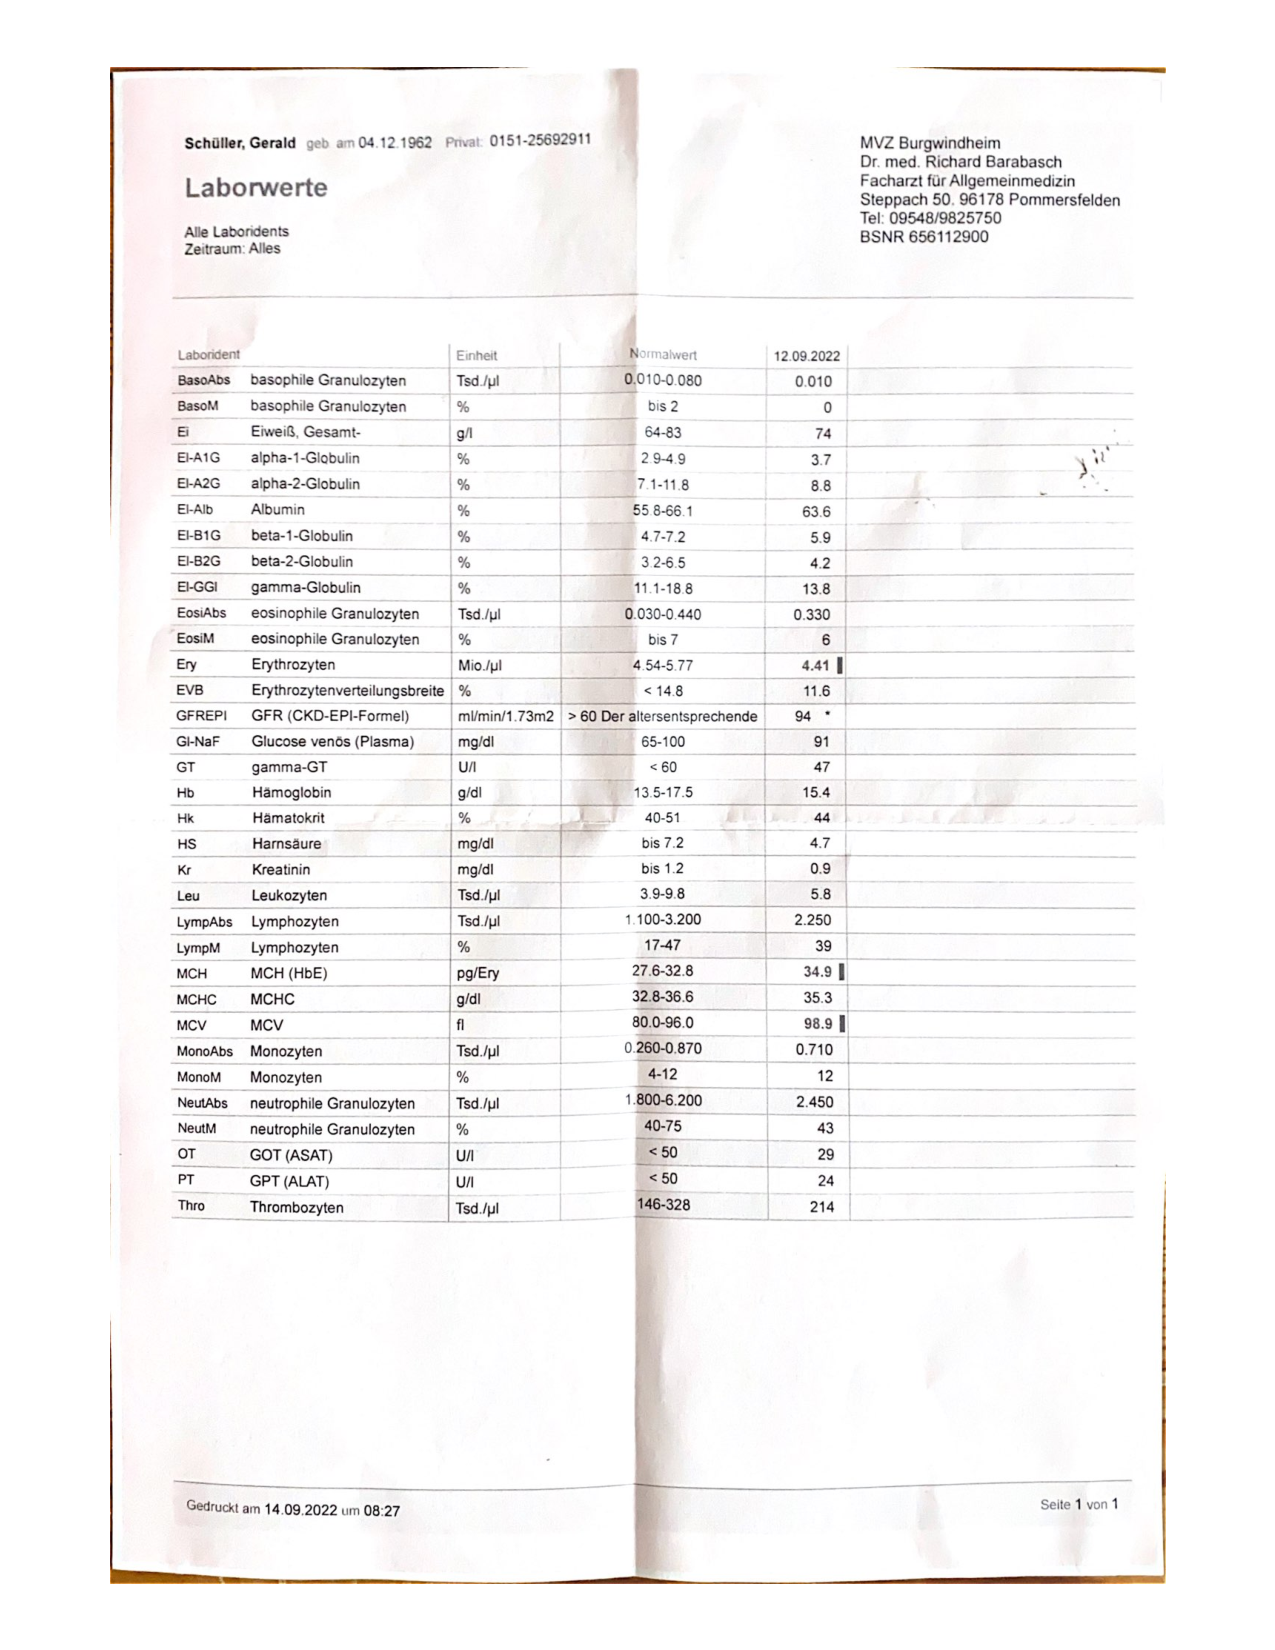
\includepdf[pages=-, scale=0.9, offset=0 0, pagecommand={%
    \begin{flushleft}  
        \section{Appendix}
      \end{flushleft} 
    \subsection{Laborwerte - 12.09.2022}\thispagestyle{plain}}
]{lw220912.pdf}

% Include the next pdf file.
% 
\includepdf[pages=-, scale=0.9, offset=0 0, pagecommand={%
%    \subsection{Ludwig Wittgenstein, Tractatus}\thispagestyle{plain}}
% ]{tractatus.pdf}


\subsection{Charaktereigenschaften}

\verb+https://wortwuchs.net/charaktereigenschaften/+


\subsection{Tractatus}

\verb+https://www.mathebibel.de/funktionen+ \\
\verb+https://home.mathematik.uni-freiburg.de/wolke/Schuster_Skript.pdf+ \\
\verb+http://www.fb10.uni-bremen.de/khwagner/grundkurs2/kapitel3.aspx+ \\
\verb+https://ftp.agdsn.de/pub/mirrors/latex/dante/fonts/stix/doc/stix.pdf+


\subsection{Das Hirtenbüblein.}

\verb+https://de.wikisource.org/wiki/Das_Hirtenb%C3%BCblein_(1857)+

\vskip 4pt
Es war einmal ein Hirtenbübchen, das war wegen seiner weisen Antworten, die es
auf alle Fragen gab, weit und breit berühmt. Der König des Landes hörte auch
davon, glaubte es nicht und ließ das Bübchen kommen. Da sprach er zu ihm
,,kannst du mir auf drei Fragen, die ich dir vorlegen will, Antwort geben, so
will ich dich ansehen wie mein eigen Kind, und du sollst bei mir in meinem
königlichen Schloß wohnen.'' Sprach das Büblein ,,wie lauten die drei Fragen?''
Der König sagte ,,die erste lautet wie viel Tropfen Wasser sind in dem
Weltmeer?'' Das Hirtenbüblein antwortete ,,Herr König, laßt alle Flüsse auf der
Erde verstopfen, damit kein Tröpflein mehr daraus ins Meer lauft, das ich nicht
erst gezählt habe, so will ich euch sagen, wie viel Tropfen im Meere sind.''
Sprach der König ,,die andere Frage lautet wie viel Sterne stehen am Himmel?''
Das Hirtenbübchen sagte ,,gebt mir einen großen Bogen weiß Papier,'' und dann
machte es mit der Feder so viel feine Punkte darauf, daß sie kaum zu sehen und
fast gar nicht zu zählen waren und einem die Augen vergiengen, wenn man darauf
blickte. Darauf sprach es ,,so viel Sterne stehen am Himmel, als hier Punkte auf
dem Papier zählt sie nur.'' Aber niemand war dazu im Stand. Sprach der König
,,die dritte Frage lautet wie viel Secunden hat die Ewigkeit?'' Da sagte das
Hirtenbüblein ,,in Hinterpommern liegt der Demantberg, der hat eine Stunde [284]
in die Höhe, eine Stunde in die Breite und eine Stunde in die Tiefe; dahin kommt
alle hundert Jahr ein Vögelein und wetzt sein Schnäblein daran, und wenn der
ganze Berg abgewetzt ist, dann ist die erste Secunde von der Ewigkeit vorbei.''

\vskip 4pt
Sprach der König ,,du hast die drei Fragen aufgelöst wie ein Weiser und sollst
fortan bei mir in meinem königlichen Schlosse wohnen, und ich will dich ansehen
wie mein eigenes Kind.“


\subsection{Grundsteuer}

\subsubsection{Bibliographie}

\verb+https://de.wikipedia.org/wiki/Grundsteuer+ \\
\verb+https://www.bundesfinanzministerium.de/Content/DE/FAQ/faq-die-neue-grundsteuer.html+ \\
\verb+https://www.elster.de/eportal/start+

\subsubsection{Definitionen}

\begin{mdframed}[style=daystyle, leftmargin=-25pt]
  \begin{itemize}
    \setlength\itemsep{-3pt}
  \item {\emps {Grundsteuer}} (Bodenzins) ist eine Geldleistung für ein
    Eigentum an einem Teil der Erdoberfläche, das im Grundbuch beschrieben wird.
  \end{itemize}
\end{mdframed}

\subsubsection{Grundsteuererklärung}

\begin{enumerate}[label={\Square}]
    \setlength\itemsep{-3pt}
  
  \item Das Dokument muss ich bis zum 31.10.2022 abgeben.
  \item Die Erklärung muss ich elektronisch über das ELSTER-Portal an das
    Finanzamt übermitteln.
  \item Ein ELSTER-Zertifikat erhalte ich unter \verb+https://www.elster.de/eportal/start+
  \item Für das ELSTER-Login benötige ich eine Zertifikationsdatei und ein Passwort.
  \item [\XBox] Zugang bekomme ich mit der steuerlichen Identifikationsnummer:
    IdNr.: 62 098 453 150; Benutzername: hozan; Lieblingsbuch: Tractatus
  \item Ich erhalte zwei Briefe: Aktivierungs-Code und Abrufcode.
  \item  [\XBox] Per EMail bestätige ich die Aktivierung meines Benutzerkontos:
    Benutzername: hozan; Aktivierungs-ID: 28287596101226690
  \item Innerhalb von 14 Tagen schickt mir das Finanzamt den Aktivierungs-Code
    postalisch.
  \item Mit dem Aktivierungs-Code kann ich die Registrierung fortsetzen.
    
\end{enumerate}

% End of a LaTeX text, that is to be printed.

\end{document}
